\documentclass[specialist, subf, href, colorlinks=true, 12pt, times, mtpro, final]{disser}

\usepackage[utf8x]{inputenc}
\usepackage[english, russian]{babel}
\usepackage[T2A]{fontenc}
\usepackage{amsmath,amsthm,amssymb}

\usepackage{enumitem}  
\usepackage{graphicx}
\usepackage{wrapfig}
\usepackage{multicol}
\usepackage{mathrsfs}
\usepackage{xcolor}
\usepackage{hyperref}
\usepackage{tikz}
\usepackage{pdfpages}
\usepackage{algorithm}
\usepackage{algpseudocode}


\usetikzlibrary{decorations.pathreplacing}
\usepackage[a4paper, mag=1000, includefoot, left=1.5cm, right=1.5cm, top=1cm, bottom=1cm, headsep=1cm, footskip=1cm]{geometry}
\usepackage{tikz}
\newcommand{\RNumb}[1]{\uppercase\expandafter{\romannumeral #1\relax}}
\usetikzlibrary{graphs}

\theoremstyle{definition}
\newtheorem{defn}{Определение}[section]
\newtheorem{example}{Пример}[section]
\newtheorem{state}{Утверждение}[section]
\newtheorem{theorem}{Теорема}[section]
\newtheorem{lemma}{Лемма}[section]
\newtheorem{axiom}{Аксиома}[section]
\newtheorem{consequence}{Следствие}[section]
\newtheorem{addition}{Примечание}[section]

\definecolor{linkcolor}{HTML}{0000ff} % цвет ссылок
\definecolor{urlcolor}{HTML}{0000ff} % цвет гиперссылок
\hypersetup{pdfstartview=FitH, linkcolor=linkcolor,urlcolor=urlcolor, colorlinks=true}

\begin{document}
\begin{titlepage}
	\begin{center}
		
		Федеральное государственное бюджетное образовательное учреждение высшего образования 
		<<Московский Государственный Университет им.\,М.\,В.\,Ломоносова>>\\
		
		\vspace{9cm}
		Механико-математический факультет
		
		{\bf Конспект лекций по курсу <<Основы механики сплошных сред>>}
		
		\vspace{9cm}
		\begin{flushright}
			{\bfРаботу выполнили студенты 510 группы}\\
		\end{flushright}
		\vspace{1cm}
		
		\normalsize Москва, 2022
	\end{center}
\end{titlepage}

	
\tableofcontents
	
\newpage
\section{Билет 1. Понятие сплошной среды. Лагранжево и эйлерово описание движения сплошной среды. Индивидуальная производная.}

\textbf{Сплошная среда} - это среда, заполняющая занятую ею область непрерывно, т.е. в любом сколь угодно малом объёме этой области содержится масса.

\textbf{Эйлеровы (пространственные) координаты} - координаты точек среды в системе координат, связанной с пространством, относительно которого происходит движения (пространственной системе координат).

\textbf{Эйлеров подход к описанию движения СС} - величины, характеризующие движение СС, рассматриваются как функции пространственных координат $x^i$ и времени t: $$\vec{f} = \vec{f}(t, x^1, x^2, x^3)$$

\textbf{Лагранжевы координаты} - параметры, которые выделяют индивидуальные точки среды.

\textbf{Лагранжев подход к описанию движения СС} - величины, характеризующие движения СС, рассматриваются как функции времени t и лагранжевых координат $\xi^i$: $$\vec{f} = \vec{f}(t, \xi^1, \xi^2, \xi^3)$$
\begin{figure}{}
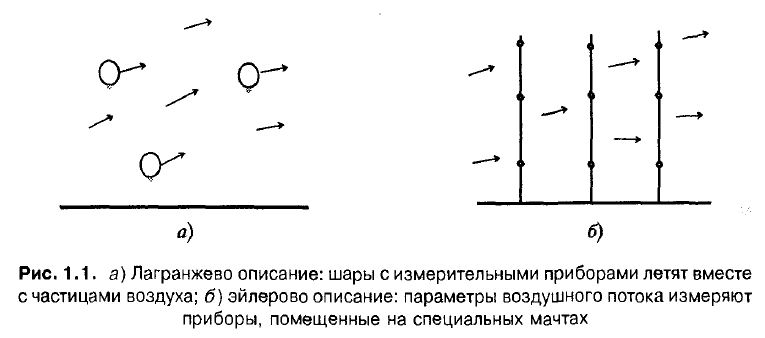
\includegraphics[width=1\textwidth]{1\t1_pic1.JPG}
\caption{\label{ris:image2}1}
\end{figure}

\textbf{Материальная (индивидуальная) производная} по времени от величины f описывает, как эта величина меняется со временем в индивидуальной точке среды. Если f задана в лагранжевом описании, то материальная производная имееет вид (для индивидуальной точки $\xi^i = const $ по определению): $$\frac{df}{dt} = \frac{\partial f(t,\vec{\xi})}{\partial t}$$

Если f задана в эйлеровом описании, то материальная производная имеет вид: $$\frac{df}{dt} = \frac{\partial f(t,\vec{x})}{\partial t} + \frac{\partial f(t, \vec{x})}{\partial x^i}\frac{\partial x^i(t,\vec{\xi})}{\partial t} = \frac{\partial f(t,\vec{x})}{\partial t} + \frac{\partial f(t, \vec{x})}{\partial x^i}v^i$$

\newpage
\section{Билет 2. Описание деформации. Тензоры Грина и Альманси. Главные оси и главные значения тензоров. Инварианты тензоров.}

\begin{center}
	\textit{\underline{Описание деформации}}
\end{center}

Деформация - это изменение длин всевозможных материальных отрезков и углов между ними. При деформациях рассмаатривают малую окрестность некоторой точки М сплошной среды. 

Рассмотрим малую частицу среды - малую окрестность некоторой произвольной точки М. Точки из малой окрестности точки М имеют в начальном состоянии координаты $x_0^i+dx_0^i$, так что если бы мы эту точку приняли за начало координат, то координаты всех точек из ее малой окрестности были бы $dx_0^i$. В конечном состоянии точка М имеет координаты $x^i$, а точки из ее окрестности $x^i+dx^i$ .
$$dx^i=\frac{\partial x^i}{\partial x_0^k}dx_0^k$$
Матрица $\left( \frac {\partial x^i}{\partial x_0^k}\right)$ - матрица дисторсии. Все преобразование чатицы, кроме поступательного переноса вместе с центром называется \textit{дисторсией}

\begin{center}
	\textit{\underline{Тензоры деформаций}}
\end{center}
Чтобы ввести тензори деформаций, удобно поначалу воспользоваться лагранжевой системой координат $\xi^i$.

Лагранжевы координаты - это параметры, которые для каждой индивидуальной точки фиксированы, це меняются, что бы с ней ни происходило. Поэтому у точки М координаты $\xi^i$ и в начальном, и в деформированном состояниях - одни и те же, и относительные координаты индивидуальных точек окрестности, то есть $d\xi^i$, -одни и те же. Конечно, это значит, что сама система координат деформируется вместе со средой. 

Тензором деформаций Грина (или лагранжевым тензором деформаций) называют тензор $$\mathring{\xi}=\xi_{ij}*\overrightarrow{\mathring{\text{э}^i}}*\overrightarrow{\mathring{\text{э}^j}}$$ где $\overrightarrow{\mathring{\text{э}^j}}$ контравариантные векторы базиса лагранжевой системы координат в начальном состоянии. 

Тензором деформаций Альмаиси (или эйлеровым тензором деформаций) называют тензор $$\hat{\xi}=\xi_{ij}*\overrightarrow{\hat{\text{э}^i}}*\overrightarrow{\hat{\text{э}^j}}$$ где $\overrightarrow{\hat{\text{э}^j}}$ контравариантные векторы базиса лагранжевой системы координат в конечном состоянии


\begin{center}
	\textit{\underline{Главные оси и главные значения тензоров.}}
\end{center}

Вводятся единичные векторы базиса $\overrightarrow{e_i}$, направленные по осям лагранжевой системы в деформированном состоянии:
$$\overrightarrow{e_i}=\frac{\overrightarrow{\text{э}_{i}}}{|\overrightarrow{\text{э}_{i}}|}=\overrightarrow{\text{э}_{i}}\sqrt{1+2\mathring{\xi_i}}$$

Система с вектораами базиса $\overrightarrow{e_i}$ будет главной для тензора Альманси. 
Связь между главными компонентами тензоров Альманси и Грина таковы:
$$\hat\xi_i=\frac{\mathring{\xi_i}}{1+2\mathring\xi_i}$$

\begin{center}
	\textit{\underline{Инварианты тензоров}}
\end{center}
Инварианты тензоров используются для получения величины относительного изменения объем $\Theta$.
При деформации параллелепипед переходит в параллелепипед с прямоугольными ребрами 
$$\theta=\sqrt{1+2\mathring{I_1}+4\mathring{I_2}+8\mathring{I_3}}-1$$
$$\theta=\sqrt{1-2\hat{I_1}+4\hat{I_2}-8\hat{I_3}}-1$$

где $\mathring{I_k},\hat{I_k}$ -первый, второй и третий инварианты тензоров Грина и Альманси:
$$I_1=\xi_1+\xi_2+\xi_3=g_{ij}\xi_{ij}$$
$$I_2=\xi_1\xi_2+\xi_2\xi_3+\xi_3\xi_1=\frac{1}{2}(I_1^2-\xi^{ij}\xi_{ij})$$
$$I3=\xi_1\xi_2\xi_3=det(\xi_j^i)$$
\newpage
\section{Билет 3. Вектор перемещения. Связь вектора перемещения и тензоров деформации. Случай малых деформаций. Геометрический смысл компонент. Относительное изменение объема. Уравнение совместности малых деформаций.}

\begin{center}
	\textit{\underline{Вектор перемещения. Связь вектора перемещения и тензоров деформации.}}
\end{center}

\begin{figure}[H]
	\centering
	\noindent\centering{
		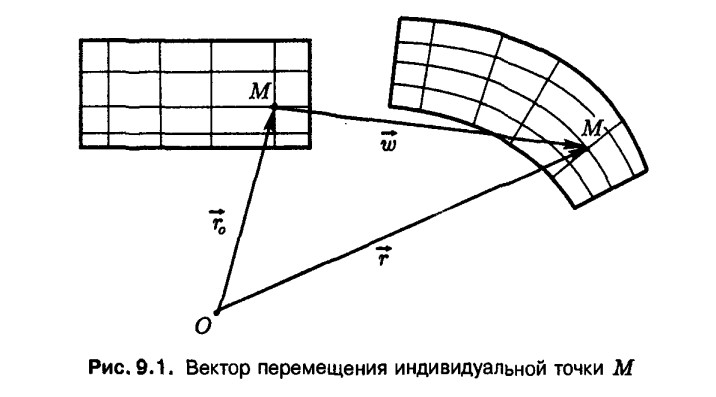
\includegraphics[width=10cm]{3/3_1.jpg}
	}
	\label{fig1}
\end{figure}

Вектор перемещений $\vec w = \vec r - \vec r_0$ - вектор, соединяющий точки, где находится индивидуальная точка среды $М$ в начальном и конечном состояниях среды.	
Лагранжевы координаты точки - её неизменные параметры, так что и в начальном, и в конечном состояниях это $\xi^i$. Продифференцируем по ним вектор перемещений:
$$
\dd{\vec w}{\xi^i} = \dd{\vec r}{\xi^i} - \dd{\vec r_0}{\xi^i} = \hat{\vec{e_i}} - \arcsup{\vec{e_i}}, \quad \text{т.е.}\quad 
\hat{\vec{e_i}} = \arcsup{\vec{e_i}} +\dd{\vec w}{\xi^i}\quad \left(\text{или} \quad  \arcsup{\vec{e_i}} = \hat{\vec{e_i}} - \dd{\vec w}{\xi^i}\right)
$$
Тогда
$$
\varepsilon_{ij} = \frac{1}{2}(\hat{g_{ij}} - \arcsup{g_{ij}}) = \frac{1}{2}((\hat{\vec{e_i}}, \hat{\vec{e_j}}) - (\arcsup{\vec{e_i}}, \arcsup{\vec{e_j}})) = \frac{1}{2}\left(\left(\arcsup{\vec{e_i}} + \dd{\vec w}{\xi^i} , \arcsup{\vec{e_j}} + \dd{\vec w}{\xi^j} \right) - (\arcsup{\vec{e_i}}, \arcsup{\vec{e_j}})\right) = \frac{1}{2}\left( \arcsup{\vec{e_i}}\dd{\vec w}{\xi^j} + \arcsup{\vec{e_j}}\dd{\vec w}{\xi^i} + \dd{\vec w}{\xi^i} \dd{\vec w}{\xi^j}\right)
$$

Вектор $w$ разложим по, соответственно, ковариантному и контравариантному базису: 
$\vec w = \arcsup{w}^k\arcsup{\vec e}_k$  и $\vec w = \arcsup{ w}_k\arcsup{\vec e}^k$. Тогда $\dd{\vec w}{\xi^i} = \nabla_i\arcsup{w}^k\arcsup{\vec e}_k = \nabla_i\arcsup{w}_k\arcsup{\vec e}^k$.

Учитывая, что $(\vec e^k,\vec e_i) = \delta_i^k$, подставим разложение $w$:
$$
\varepsilon_{ij} = \dfrac{1}{2}(\nabla_j\arcsup{w}_k(\arcsup{\vec e}^k, \arcsup{\vec e}_i) + \nabla_i\arcsup{w}_k(\arcsup{\vec e}^k, \arcsup{\vec e}_j) + \nabla_i\arcsup{w}^k \nabla_j\arcsup{w}_l(\arcsup{\vec e}_k, \arcsup{\vec e}^l)) = \dfrac{1}{2}(\nabla_j\arcsup{w}_i + \nabla_i\arcsup{w}_j + 
\nabla_i\arcsup{w}^k \nabla_j\arcsup{w}_k)
$$
(Здесь следует подставлять координаты начальной точки $\vec w = w^i(x_0^k)e_i(x_0^k)$, а можно вывести аналогичное $\varepsilon_{ij} = \dfrac{1}{2}(\nabla_j\hat {w}_i + \nabla_i\hat {w}_j + 
\nabla_i\hat {w}^k \nabla_j\hat {w}_k)$ и подставлять координаты конечной точки $\vec w = w^i(x^k)e_i(x^k)$).

\begin{center}
	\textit{\underline{Случай малых деформаций.}}
\end{center}

В случае $\nabla_i {w}^k \ll 1$, или $\nabla_i {w}_k\nabla_j {w}^k \ll \nabla_i {w}_k$, получим тензор малых деформаций $\varepsilon_{ij} = \dfrac{1}{2}(\nabla_j {w}_i + \nabla_i {w}_j)$.

$\hat{\vec{e_i}} = \arcsup{\vec{e_i}} +\dd{\vec w}{\xi^i} = \hat{\vec{e_i}} = \arcsup{\vec{e_i}} +\nabla_i\arcsup{w}^k\arcsup{\vec e}_k = (\delta_i^k + \nabla_i\arcsup{w}^k)\arcsup{\vec{e_i}}$, откуда видно, что из малости производных перемещений следует малость деформаций. Обратное неверно, так как относительные перемещения могут быть большими даже при малых деформациях, если относительные повороты отрезков не малы (тело, размеры которого во всех направлениях не одного порядка: пластинки, оболочки, стержни). Согнем металлическую линейку, она практически не растягивается, но ее элементы поворачиваются друг относительно друга:
\begin{figure}[H]
	\centering\noindent{
		
\includegraphics[width=10cm]{3/3_2.jpg}
	}
	\label{fig2}
\end{figure}

\begin{center}
	\textit{\underline{Геометрический смысл компонент.}}
\end{center}

По определению скалярного произведения: $\hat g_{ij} = (\hat{\vec{e_i}}, \hat{\vec{e_j}}) = |\hat{\vec{e_i}}||\hat{\vec{e_j}}|\cos\psi_{ij}, \quad \arcsup g_{ij} = (\arcsup{\vec{e_i}}, \arcsup{\vec{e_j}}) = |\arcsup{\vec{e_i}}||\arcsup{\vec{e_j}}|\cos\arcsup\psi_{ij}$, где $\psi_{ij}, \arcsup\psi_{ij}$ - углы между векторами базиса лагранжевой системы координат в начальном и конечном состояниях. Отсюда
$$
\varepsilon_{ij} = \frac{1}{2}(|\hat{\vec{e_i}}||\hat{\vec{e_j}}|\cos\psi_{ij} - |\arcsup{\vec{e_i}}||\arcsup{\vec{e_j}}|\cos\arcsup\psi_{ij}).
$$

Коэффициент относительного удлинения малого отрезка: $e = \dfrac{ds - ds_0}{ds_0}$

\noindent
\parbox[b][4cm][t]{10mm}{
	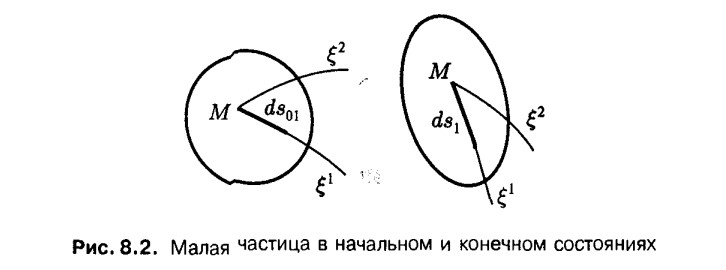
\includegraphics[height=3.75cm]{3/3_3.jpg}}
\hfill
\parbox[b][4cm][t]{68mm}{
	Бесконечно малый вектор вдоль $\xi^1: d\vec r_0 = d\xi^1\arcsup{\vec{e_1}}$. 
	
	Его длина $ds_{01} = d\xi^1|\arcsup{\vec{e_1}}|$.
	
	При деформации перейдет в вектор: $d\vec r = d\xi^1\hat{\vec{e_1}}$. 
	
	Его длина $ds_{1} = d\xi^1|\hat{\vec{e_1}}|$.
	
	
}

\hfill

$e_1 = \dfrac{ds_1 - ds_{01}}{ds_{01}} = \dfrac{d\xi^1|\hat{\vec{e_1}}| - d\xi^1|\arcsup{\vec{e_1}}|}{d\xi^1|\arcsup{\vec{e_1}}|} = \dfrac{|\hat{\vec{e_1}}|}{|\arcsup{\vec{e_1}}|} - 1$. Аналогично, $e_i = \dfrac{|\hat{\vec{e_i}}|}{|\arcsup{\vec{e_i}}|} - 1$, $i = 1,2,3$.

Отсюда $|\hat{\vec{e_i}}| = (1+e_i)|\arcsup{\vec{e_i}}|$. Тогда

$$
\varepsilon_{ij} = \dfrac{1}{2}((1+e_i)(1+e_j)\cos\psi_{ij} - \cos\arcsup\psi_{ij})|\arcsup{\vec{e_i}}||\arcsup{\vec{e_j}}|.
$$

\begin{itemize}	
	\item При $i = j$: Т.к. $\psi_{ij} = 0 = \arcsup\psi_{ij}$, то 
	$\varepsilon_{ii} = \dfrac{1}{2}((1+e_i)^2 - 1)|\arcsup{\vec{e_i}}|^2 = (e_i + \dfrac{1}{2}e_i^2)|\arcsup{\vec{e_i}}|^2$.
	Если отсчетная система декартова (т.е. $|\arcsup{\vec{e_i}}| = 1$): $\varepsilon_{ii} = (e_i + \dfrac{1}{2}e_i^2)$. Если, к тому же, деформации малы (т.е. $\dfrac{1}{2}e_i^2 \ll e_i$), то $\varepsilon_{ii} = e_i$. (т.е.в случае малых деформаций диагональные элементы - это коэффициенты относительного удлинения материальных отрезков, лежащих вдоль координатных осей).
	\item При $i \not= j$: Если отсчетная система декартова (т.е. $|\arcsup{\vec{e_i}}| = 1, \arcsup\psi_{ij} = \dfrac{\pi}{2}$), введем $\chi_{ij} = \arcsup\psi_{ij} - \psi_{ij} = \dfrac{\pi}{2} - \psi_{ij}$. Тогда $\varepsilon_{ij} = \dfrac{1}{2}(1+e_i)(1+e_j)\sin{\chi_{ij}}$. Если, к тому же, деформации малы (т.е. $e_i \ll 1, \sin \chi_{ij} \approx \chi_{ij}$): $\varepsilon_{ij} = \dfrac{1}{2}\chi_{ij}$. (т.е. в случае малых деформаций внедиагональные элементы - это половина изменения угла между материальными отрезками, лежащими вдоль координатных осей).
\end{itemize}

Если $\varepsilon_{ij} = 0$, то $\chi_{ij} = 0$ и $\psi_{ij} = \dfrac{\pi}{2}$, т.е. в результате деформации углы между координатными осями остаются ортогональныим.

\begin{center}
	\textit{\underline{Относительное изменение объема.}}
\end{center}

Возьмем в качестве начальной лагранжевой системы главную систему для тензора Грина, т.е. 
$$
\arcsup g_{ij} = 
\begin{pmatrix} 
1 & 0 & 0 \\
0 & 1 & 0 \\
0 & 0 & 1 
\end{pmatrix},
\varepsilon_{ij} = 
\begin{pmatrix} 
\varepsilon_{11} & 0 & 0 \\
0 & \varepsilon_{22} & 0 \\
0 & 0 & \varepsilon_{33}
\end{pmatrix} = 
\begin{pmatrix} 
\arcsup\varepsilon_{1} & 0 & 0 \\
0 & \arcsup\varepsilon_{2} & 0 \\
0 & 0 & \arcsup\varepsilon_{3}
\end{pmatrix}
\Rightarrow
\hat g_{ij} = 
\begin{pmatrix} 
1+2\arcsup\varepsilon_{1} & 0 & 0 \\
0 & 1+2\arcsup\varepsilon_{2} & 0 \\
0 & 0 & 1+2\arcsup\varepsilon_{3}
\end{pmatrix}
$$
(последняя матрица получена из $\varepsilon_{ij} = \frac{1}{2}(\hat{g_{ij}} - \arcsup{g_{ij}})$). Т.е. в деформированном состоянии лагранжева система ортогональна, $\varepsilon_{ij}$ - диагональна.

Отсюда 
$$ |\hat{\vec{e_i}}| = \sqrt{g_{ii}} = \sqrt{1 + 2\arcsup\varepsilon_{i}} = (1+e_i)|\arcsup{\vec{e_i}}| = (1+e_i)
$$
Рассмотрим малую частицу среды, имевшую в начальном состоянии форму прямоугольного параллелепипеда, построенного на векторах $d\xi^1\arcsup{\vec{e_1}}$, $d\xi^2\arcsup{\vec{e_2}}$, $d\xi^3\arcsup{\vec{e_3}}$. Его объем $dV_0 = d\xi^1d\xi^2d\xi^3$. Т.к. $\varepsilon_{ij} = 0$ при $i \not= j$, то деформированный параллелепипед тоже прямоугольный с ребрами $d\xi^1\hat{\vec{e_1}}$, $d\xi^2\hat{\vec{e_2}}$, $d\xi^3\hat{\vec{e_3}}$. Его объем $dV = |\hat{\vec{e_1}}||\hat{\vec{e_2}}||\hat{\vec{e_3}}|d\xi^1d\xi^2d\xi^3$.
\begin{figure}[H]
	\centering\noindent{
		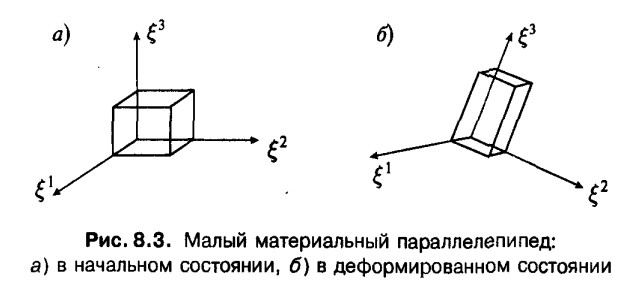
\includegraphics[width=10cm]{3/3_4.jpg}
	}
	\label{fig4}
\end{figure}
Относительное изменение объема $\theta = \dfrac{dV - dV_{0}}{dV_{0}} = \sqrt{(1+2\arcsup\varepsilon_{1})(1+2\arcsup\varepsilon_{2})(1+2\arcsup\varepsilon_{3})} - 1 = (1+e_1)(1+e_2)(1+e_3) - 1$. В случае малых деформаций: $\theta \approx e_1 + e_2 + e_3 = \sum\varepsilon_{ii} = \sum\nabla_iw^i = div {\vec w}$.


\begin{center}
	\textit{\underline{Уравнение совместности малых деформаций.}}
\end{center}

В декартовой системе $\varepsilon_{ij} = \dfrac{1}{2}\left(\dd{w_i}{x^j}+ \dd{w_j}{x^i}\right)$. Используя обозначения $\dd{\varepsilon_{ij}}{x^k} = \varepsilon_{ij, k}$, продифференцируем:
\begin{gather*}
\varepsilon_{ij, kl} = \dfrac{1}{2}(w_{i,jkl} + w_{j,ikl}) \\
\varepsilon_{kl, ij} = \dfrac{1}{2}(w_{k,lij} + w_{l,kij}) \\
\varepsilon_{il, jk} = \dfrac{1}{2}(w_{i,ljk} + w_{l,ijk}) \\
\varepsilon_{jk, il} = \dfrac{1}{2}(w_{j,kil} + w_{k,jil}) \\
\end{gather*}
Из непрерывности перемещений: $\varepsilon_{ij, kl} + \varepsilon_{kl, ij} - \varepsilon_{il, jk} - \varepsilon_{jk, il} = 0$. Здесь 81 уравнение (рассматривается трехмерное пространство), из которых только 6 независимые (в силу симметричности компонент тензора деформации и равенства смешанных производных):
\begin{gather*}
2\varepsilon_{12, 12} = \varepsilon_{11, 22} + \varepsilon_{22, 11} \\
2\varepsilon_{13, 13} = \varepsilon_{11, 33} + \varepsilon_{33, 11} \\
2\varepsilon_{23, 23} = \varepsilon_{22, 33} + \varepsilon_{33, 22} \\
\varepsilon_{11, 23} = \dd{}{x^1}(-\varepsilon_{23, 1} + \varepsilon_{13, 2} + \varepsilon_{12, 3}) \\
\varepsilon_{22, 13} = \dd{}{x^2}(-\varepsilon_{13, 2} + \varepsilon_{21, 3} + \varepsilon_{23, 1}) \\
\varepsilon_{33, 12} = \dd{}{x^3}(-\varepsilon_{12, 3} + \varepsilon_{23, 1} + \varepsilon_{13, 2})
\end{gather*}
\newpage
\section{Билет 4. Тензор скоростей деформации. Его связь с полем скоростей. Кинематический смысл компонент тензора скоростей деформации. Дивиргенция скорости.}

\begin{center}
	\textit{\underline{Определение}}
\end{center}

Введем тензор скоростей деформаций. Используем Лагранжеву систему координат $\xi^{i}$, рассмотрим точку и небольшую ее окрестность. Рассмотрим малые деформации, которые произошли с этой окрестностью за время $\Delta t$. Для таких деформаций начальным является момент времени $t$, а конечным $t + \Delta t$. Тогда тензор деформаций примет вид: 

$$
\Delta \varepsilon_{ij} = \varepsilon_{ij} (t + \Delta t, \xi^i) - \varepsilon_{ij} (t, \xi^i) = \frac{1}{2} \left(\hat g_{ij}(t + \Delta t, \xi) - g_{ij}^0(\xi)  \right) - \frac{1}{2}
\left(\hat g_{ij}(t, \xi) - g_{ij}^0(\xi) \right) = \frac{1}{2} \left(\hat g_{ij}(t + \Delta t, \xi) - \hat g_{ij}(t, \xi)  \right)
$$

Определение: Рассмотрим предел отношения приращения деформаций к промежутку времени: $lim_{\Delta t \rightarrow 0} \frac{\Delta \varepsilon}{\Delta t} = e_{ij}$,
где $e_{ij}$ - компоненты тензора скоростей деформаций.

Рассмотрим ранее расписанное приращение $\Delta \varepsilon_{ij}$ и подставим в его определение тензора скоростей деформаций. В итоге получим:

$$e_{ij} = \frac{d \hat g_{ij}}{d t}$$

\begin{center}
	\textit{\underline{Выражение компонент тензора через компоненты вектора скорости}}
\end{center}
Вспомним, что $\varepsilon_{ij} = \frac{1}{2} \left(\nabla_{i}w_{j} + \nabla_{j}w_{i} \right)$ (Или в нотации частных производных: $\frac{1}{2} \left(\partial_{i}w_{j} + \partial_{j}w_{i} \right)$). Пусть вектор перемещений $\overrightarrow{w} = \overrightarrow{v} \Delta t$, тогда имеем:

$$\Delta \varepsilon_{ij} = \frac{1}{2} \left(\nabla_{i}\Delta w_{j} + \nabla_{j}\Delta w_{i} \right)$$

Так как $v_{i} = \lim\limits_{\Delta t \rightarrow 0} \frac{\Delta w_{i}}{\Delta t}$, то получаем:

$$e_{ij} = \frac{1}{2} \left(\nabla_{i}v_{j} + \nabla_{j}v_{i}\right)$$

\begin{center}
	\textit{\underline{Кинематический смысл}}
\end{center}
Механический смысл компонент тензора скоростей деформаций в декартовой системе следует из формулы $e_{ij} = \lim\limits_{\Delta t \rightarrow 0} \frac{\varepsilon_{ij}}{\Delta t}$. Ранее было показано, что диагональные компоненты тензора малых деформаций равны коэффициентам относительного удлинения отрезков, лежавших до деформации вдоль соответствующих осей (если система координат декартова). Следовательно, механический смысл диагональных компонент тензора скоростей деформаций - скорость удлинения (сокращения) отрезка. Аналогично, вне диагональные элементы - половина скоростей изменения углов между отрезками. 

\begin{center}
	\textit{\underline{Дивергенция скорости}}
\end{center}
Так как $\varepsilon_{ii} = \frac{1}{2} \left(\nabla_{i}v_{i} + \nabla_{i}v_{i} \right) = \nabla_{i}v_{i}$
$$div \overrightarrow{v} = \sum\limits_{i} \nabla_{i} v^i = \sum\limits_{i} \varepsilon^{i}_{i}$$
\input {5/5_ticket.tex}
\newpage
\section{Билет 6. Производная по времени от интеграла по подвижному объему. Уравнение неразрывности в переменных Эйлера и Лагранжа.}
\begin{center}
    \textit{\underline{Закон сохранения массы для индивидуального объема сплошной среды}}
\end{center}

Закон сохранения массы утверждает, что \textbf{масса M любого индивидуального объема сплошной среды постоянна}:
\begin{center}$
M = const
$\end{center}
\textbf{Индивидуальным объемом} называют выделенную часть среды, состоящую из одних и тех же индивидуальных частиц. В механике сплошных сред интерес представляет не столько масса некоторогообъема, сколько распредление массы по объему, которое характеризируется распределением плотности. Определим понятие плотности. Рассмотрим малый объем $\Delta {V}$ с массой $\Delta m$. Средняя плотность этого объема равна:
\begin{center}$
\rho_{ср} = \frac{\Delta m}{\Delta V}
$\end{center}

Плотность $\rho$ в точке среды определяется как предел этого отношения, когда $\Delta V$ стягивается в рассматриваемую точку:
\begin{center}$
\rho = \lim\limits_{\Delta V \to 0} \frac{\Delta m}{\Delta V}
$\end{center}

Масса в объеме $V$ равна:
\begin{center}$
M = \int\limits_V \rho dV
$\end{center}

\textbf{Закон сохранения массы для конечного индивидуального объема сплошной среды $V_{инд}$} гласит:
\begin{center}$
\frac{d}{dt} \int\limits_{V_{инд}(t)} \rho dV = 0
$\end{center}

$V_{инд}(t)$ - индивидуальный, в общем случае, подвижный объем.

\begin{center}
    \textit{\underline{Производная по времени от интеграла по подвижному индивидуальному объему}}
\end{center}
Выведем формулу дифференцирования по времени интеграла по подвижному объему $V(t)$ от некоторой величины $A(x^i, t)$. По определния производной имеем:
\begin{center}$
\frac{d}{dt} \int\limits_{V(t)} A(x^i,t) dV =
\lim\limits_{\Delta t \to 0} \frac{\int\limits_{V(t + \Delta t)} A(x^i,t + \Delta t)dV - \int\limits_{V(t)}A(x^i,t)dV}{\Delta t}
$\end{center}
В правой части вычтем и прибавим одно и то же слагаемое:
\begin{center}$
\int\limits_{V(t + \Delta t)} A(x^i, t)dV
$\end{center}
Тогда получим
\begin{center}$
\frac{d}{dt} \int\limits_{V(t)} A(x^i,t) dV
=\newline
\lim\limits_{\Delta t \to 0} \frac{\int\limits_{V(t + \Delta t)} A(x^i,t + \Delta t)dV - \int\limits_{V(t + \Delta t)}A(x^i,t)dV}{\Delta t}
+
\lim\limits_{\Delta t \to 0} \frac{\int\limits_{V(t + \Delta t)} A(x^i,t)dV - \int\limits_{V(t)}A(x^i,t)dV}{\Delta t}
=\newline
\lim\limits_{\Delta t \to 0}\int\limits_{V(t + \Delta t)} \frac{A(x^i, t + \Delta t) - A(x^i, t)}{\Delta t}dV
+
\lim\limits_{\Delta t \to 0}\frac{1}{\Delta t}\int\limits_{V(t + \Delta t) - V(t)}A(x^i, t)dV
$\end{center}
Первое слагаемое в последней сумме равно:
\begin{center}$
\int\limits_{V(t)}\frac{\partial A}{\partial t}dV
$\end{center}
Для вычисления второго слагаемого разбиваем область $V(t + \Delta t) - V(t)$ на сумму $N$ малых цилиндров с основаниями $\Delta \sigma_k$, представляющими собой элементы поверхности $\Sigma$ объема $V(t)$, и длинами образующих $|\Vec{v}|\Delta
t$. Объем элементарного цилиндра равен произведению площади основания на высоту:
\begin{center}$
\Delta V_k = \Delta \sigma_k v_{n_k} \Delta t,
$\end{center}
где $v_{n_k}$ - проекция скорости на нормаль к площадке $\Delta \sigma_k$. Интеграл по области $V(t + \Delta t) - V(t)$ можно представить как соответсвующий предел суммы произведений значений подинтегральной функции в точках элементарных цилиндров на объемы этих цилиндров. Тогда второе слагаемое вычисляется так:
\begin{center}$
\lim\limits_{\Delta t \to 0} \frac{1}{\Delta t}\lim\limits_{N \to \infty}\sum_{k=1}^{N}A(x_k^i,t)v_{n_k}\Delta t \Delta \sigma_k
=
\int\limits_{\Sigma}Av_n d\sigma
$\end{center}
где $\Sigma$ - поверхность объема V(t)

Итак, \textbf{формула дифференцирования по времени интеграла по подвижному объему} выглядит так:
\begin{equation}
    \frac{d}{dt}\int\limits_{V(t)}A dv= \int\limits_V \frac{\partial A}{\partial t} dV + \int\limits_{\Sigma}A v_n d\sigma
\end{equation}
С использованием формулы (1) \textbf{закон сохранения массы} может быть записан в виде:
\begin{equation}
    \int\limits_V \frac{\partial \rho}{\partial t} dV + \int\limits_{\Sigma}\rho v_n d \sigma = 0
\end{equation}

\begin{center}
    \textit{\underline{Дифференциальное уравнение неразрывности - следствие закона сохранения массы}}
\end{center}
Диффренциальное уравнение, которое выводится из закона сохранения массы, называется \textbf{уравнением неразрывности}. Для вывода уравнения неразрывности нужно преобразовать поверхностный интеграл в соотношении (2) в объемный. Пусть $\rho, \Vec{v}$ непрерывны и дифференцируемы в $V$. Применяем формулу Гаусса-Остроградского. В декартовой системе координат имеем
\begin{center}$
\int\limits_{\Sigma} \rho v_n d \sigma
= \int\limits_{\Sigma} (\rho v_x cos \hat{(n,x)} + \rho v_y cos \hat{(n,y)} + \rho v_z cos \hat{(n,z)})d \sigma
=\newline
\int\limits_V ( \frac{\partial \rho v_x}{\partial x} + \frac{\partial \rho v_y}{\partial y} + \frac{\partial \rho v_z}{\partial z})dV
=
\int\limits_V (div \rho \Vec{v})dV
$\end{center}
Следовительно, для непрерывного движения закон сохранения массы может быть записан в виде:
\begin{center}$
\int\limits_V (\frac{\partial \rho}{\partial t} + div \rho \Vec{v})dV = 0
$\end{center}
Так как это равенство должно выполняться для любого объема, то если подынтегральное выражение непрерывно, то оно должно равняться нулю. Получаем
\textbf{уравнение неразрывности при эйлеровом описании}:
\begin{equation}
    \frac{\partial \rho}{\partial t} + div (\rho \Vec{v}) = 0
\end{equation}
Напомним, что в произвольной системе координат
\begin{center}$
div \rho \Vec{v} = \nabla_i(\rho v^i)
$\end{center}
В декартовых координатах уравнение неразрывности записывается так:
\begin{center}$
\frac{\partial \rho}{\partial t} + \frac{\partial \rho v_x}{\partial x} + \frac{\partial \rho v_y}{\partial y} + \frac{\partial \rho v_z}{\partial z} = 0
$\end{center}
или
\begin{center}$
\frac{\partial \rho}{\partial t} + v_x \frac{\partial \rho}{\partial x} + v_y \frac{\partial \rho}{\partial y} + v_z \frac{\partial \rho}{\partial z} + \rho div (\Vec{v}) = 0
$\end{center}
Полная (ииндивидуальная) производная по времени $\frac{d \rho}{d t}$ определяется формулой
\begin{center}$
\frac{d \rho}{d t} = \frac{\partial \rho}{\partial t} + v_x \frac{\partial \rho}{\partial x} + v_y \frac{\partial \rho}{\partial y} + v_z \frac{\partial \rho}{\partial z}
$\end{center}
поэтому \textbf{уравнение неразрывности} можно записать так:
\begin{equation}
    \frac{d \rho}{d t} + \rho div(\Vec{v}) = 0
\end{equation}
Уравнения (3) и (4) представляют собой две различные формы уравнения неразрывности в эйлеровых переменных.

\begin{center}
    \textit{\underline{Уравнение неразрывности в лагранжевых координатах}}
\end{center}
Уравнение неразрывности следует из закона сохранения массы. В эйлеровых (пространственных) координатах оно имеет вид:
\begin{equation}
    \frac{d \rho}{d t} + \rho div(\Vec{v}) = 0
\end{equation}
где
\begin{center}$
\frac{d \rho}{d t} = \frac{\partial \rho}{\partial t} + v^k \nabla_k \rho,
\nabla_k \rho = \frac{\partial \rho}{\partial x^k}
$\end{center}
В лагранжевых координатах $\xi^i$ индивидуальная производная плотности по времени есть просто частная производная:
\begin{center}$
\frac{d \rho}{d t}  = \frac{\partial \rho (t, \xi)}{\partial t}
$\end{center}
(через $\xi$ обозначен набор $\xi^1$, $\xi^2$, $\xi^3$). Поэтому уравнение (5) записывается в лагранжевых координатах так:
\begin{equation}
    \frac{\partial \rho (t, \xi)}{\partial t} + \rho div(\Vec{v}) = 0
\end{equation}
Это один из видов уравнения неразрывности в лагранжевых координатах.
\newpage
\section{Билет 7. Изменение количества движения конечного объема сплошной среды. Массовые и поверхностные силы. Вектор напряжения. Тензор напряжения. Механический смысл его компонент. Изменение момента количества движения}

\textit{\underline{Массовые силы}} - это силы распределённые по объему $V$. Пример: сила тяжести, гравитационные силы, силы инерции.

\textit{\underline{Поверхностные силы}} - это силы распределённые по поверхности сплошной среды. Например, если налить жидкость в стакан, то на поверхности $S$ соприкосновения жидкости со стенками сосуда будет наблюдаться силовое взаимодействие.

Если разделить объем $V$ сечением $S$ на два объема: $V_1$ и $V_2$, и если рассматривать движение одной из его частей, например $V_1$, то необходимо заменить $V_2$ массовыми силами, распределенными по $V_1$ и поверхностными, распределенными по $S$. Возьмем, некоторую точку $M$ внутри тела и рассмотрим в этой точке различные площадки $d\sigma$. Полную силу действующую со стороны $V_2$ на объем $V_1$ на площадке $d\sigma$ с нормалью $n$, обозначим через $d\vec{P}$. Пусть $d\vec{P} = \vec{p_n}d\sigma$. Такого рода поверхностные силы можно вводить в любой точке сплошной среды, они называются силами внутренних напряжений. 

В каждой такой точке $M$ сплошной среды существует бесконечно много векторов $\vec{p_n}$, соответствующих бесконечному набору площадок $d\sigma$. Однако между ними существует универсальная, не зависящая от частных свойств движущейся среды, связь:

\begin{center}
    \textit{\underline{Уравнение количества движения для конечного объема сплошной среды}}
\end{center}
$$
\frac{d}{dt}  \int_{V} \vec{v} \rho \,d\tau =  \int_{V} \vec{F} \rho \,dV  + \int_{\Sigma} \vec{p_n} \,d\sigma
$$

Выводится оно из уравнения количества движения для системы точек, которое обобщается из уравнения Ньютона для одной материальной точки:
$$
m \frac{d\vec{v}}{dt} = \frac{dm\vec{v}}{dt} = \vec{F}
$$
Если у нас система материальных точек:
$$
\frac{dm_i\vec{v_i}}{dt} = \vec{F_i}
$$
Где $F_i$ это все силы: и внешние, и внутренние. Тогда сложив эти уравнения получим:
$$
\sum_{i = 1}^{n} \frac{dm_i\vec{v_i}}{dt} = \sum_{i = 1}^{n} \vec{F^{(e)}_i}
$$
где справа стоит сумма только внешних сил, ибо внутренние попарно сократятся. 
$$
Q = \sum_{i = 1}^{n} m_i \vec{v_i} 
$$
называется количество движения системы. Обобщив это уравнение для конечного объема $V$, ограниченного поверхностью $\Sigma$, получим нужное нам уравнение количества движения для конечного объема сплошной среды:
$$
\frac{d}{dt}  \int_{V} \vec{v} \rho \,d\tau =  \int_{V} \vec{F} \rho \,dV  + \int_{\Sigma} \vec{p_n} \,d\sigma
$$
Вернёмся к вектору напряжений. Если рассмотреть уравнение количества движения для сколь угодно малого объема, то можно получить зависимость напряжения $\vec{p_n}$ на произвольной площадке $d\sigma$ от векторов напряжений $\vec{p^1}, \vec{p^2}, \vec{p^3}$ на координатных площадках:
$$
\vec{p_n} = \vec{p}^i\vec{n_i} = p^{ki}\vec{e_k}(\vec{e_i}\vec{n})
$$
Это равенство задаёт координаты \textit{\underline{тензора внутренних напряжений}} $P = p^{ki}\vec{e_k}\vec{e_i}$

\begin{center}
    \textit{\underline{Изменение момента количества движения}}
\end{center}
    Аналогично уравнению изменения количества движения, выводится и уравнение изменения момента количества движения.
    Умножив векторно слева на радиус-вектор $r$ получается уравнение моментов количества движения для одной материальной точки:
$$
\frac{d\vec{K}}{dt} = \vec{\mathfrak{M}}
$$
где $\vec{K} = [\vec{r} \times m\vec{v}]$ и $\vec{\mathfrak{M}} = [\vec{r} \times \vec{F}]$. Для системы получим:
$$
\frac{d\vec{K}}{dt} = \sum_{i=1}^{n}\vec{r_i}\times\vec{F_i^{(e)}}
$$
В классическом случае моментом количества движения объема V сплошной среды обычно называют 
$$
\vec{K} = \int_{V} (\vec{r} \times \vec{v}) \rho d \vec{\tau}
$$
И уравнение моментов количества движения запишется тогда как:
$$
\frac{d}{dt} \int_{V} (\vec{r} \times \vec{v}) \rho d\vec{\tau} = \int_{V} (\vec{r} \times \vec{F}) \rho d\vec{\tau} + \int_{\Sigma} (\vec{r} \times \vec{p_n}) \rho d\sigma
$$

Если на тело внешние силы не действуют, то очевидно, что момент количества движения постоянен
\newpage
\section{Билет 8. Дифференциальные уравнения движения сплошной среды и момента количества движения. Симметрия тензора напряжения. Теорема живых сил.}
\subsection{Дифференциальные уравнения движения}
Закон сохранения количества движения: 
$$\frac{d}{dt}  \int_{V} \rho \vec{v} \,dV =  \int_{V} \rho \vec{F} \,dV  + \int_{\Sigma} \vec{P_n} \,d\sigma $$

$\vec{P_n} =  p^{ij}n_j \vec{e_i}$ - подставим это в правую часть и преобразуем последнее слагаемое по теореме Гаусса-Остроградского: 

 % $$ \int_{\Sigma} \vec{P_n} \,d\sigma = \int_{\Sigma} p^{ij}n_j \vec{e_i} \,d\sigma $$


$$\int_{\Sigma} p^{ij}n_j \vec{e_i} \,d\sigma = \int_{V} \nabla_j p^{ij} \vec{e_i}  \,dV \ \Rightarrow$$

 $$\int_{V} (\rho \frac{d \vec{v}}{dt} -  \rho \vec{F}   -  \nabla_j p^{ij} \vec{e_i} ) \,dV = 0 \Rightarrow$$

Подынтегральное выражение равно нулю - это и есть дифференциальные уравнения движения: 

$$\rho \frac{d \vec{v}}{dt} =  \rho \vec{F}   +  \nabla_j p^{ij} \vec{e_i} $$

\subsection{Дифференциальные уравнения момента количества движения}
Закон сохранения момента количества движения: 

$$\frac{d}{dt} ( \int_{V} \rho [\vec{r} \times \vec{v}] \,dV +   \int_{V} \rho \vec{k} \,dV )  =  \int_{V} \rho [\vec{r} \times \vec{F}] \,dV  +  \int_{V} \rho \vec{h} \,dV + \int_{\Sigma} [\vec{r} \times \vec{P_n}] \,d\sigma + \int_{\Sigma} \vec{M_n} \,d\sigma $$

Преобразуем левую часть: 
$$\frac{d}{dt} ( \int_{V} \rho [\vec{r} \times \vec{v}] \,dV +   \int_{V} \rho \vec{k} \,dV ) = \int_{V} \rho ([\vec{r} \times \frac{d\vec{v}}{dt}] + [\frac{d\vec{r}}{dt} \times \vec{v}] +  \frac{d \vec{k}}{dt} \big ) \,dV  $$

Так как  $[\frac{d\vec{r}}{dt} \times \vec{v}] =  [\vec{v} \times \vec{v}] = 0$, то левая часть принимает следующий вид: 

$$\int_{V} \rho ([\vec{r} \times \frac{d\vec{v}}{dt}] +  \frac{d \vec{k}}{dt} \big ) \,dV  $$

Преобразуем правую часть с помощью теоремы Гаусса - Остроградского (аналогично дифф. уравн.): 

\begin{itemize}
    \item $\int_{\Sigma} [\vec{r} \times \vec{P_n}] \,d\sigma = \int_{\Sigma} [\vec{r} \times \vec{P^k}]n_k \,d\Sigma =  \int_{V} \nabla_k[\vec{r} \times \vec{P^k}] \,d\sigma  $

    \item $ \int_{\Sigma} \vec{M_n} \,d\sigma = \int_{\Sigma} \vec{M^k}n_k \,d\sigma = \int_{V} \nabla_k\vec{M_k} \,dV $
\end{itemize}

Подставим все в закон сохранения момента количества движения и занесем все под один интеграл по объему V, приравниваем подынтегральное выражение к 0 и получаем дифференциальные уравнения момента количества движения: 
$$ \rho ([\vec{r} \times \frac{d\vec{v}}{dt}] + \frac{d \vec{k}}{dt}) =   \rho ( [\vec{r} \times \vec{F}]  +  \vec{h} ) + \nabla_k[\vec{r} \times \vec{P^k}] + \nabla_k \vec{M^k}  $$

Далее используем уравнения движения: заменяем $\frac{d\vec{v}}{dt}$ на $\rho \vec{F}   +  \nabla_k \vec{P^k} $ и получаем упрощенное выражение: 

$$ \rho \frac{d \vec{k}}{dt} =  [(\nabla_k\vec{r}) \times \vec{P^k}] + \rho \vec{h} + \nabla_k \vec{M^k}  $$

\subsection{Симметрия тензора напряжений}
Пусть $\vec{k} = 0, \vec{h} = 0, \vec{M^k} = 0$, тогда из упрощенной формы уравнения движения: 

$$[(\nabla_k\vec{r}) \times \vec{P^k}] = 0 \Rightarrow $$

$$p^{ik}[\vec{e_k} \times  \vec{e_i}] = 0 \Rightarrow $$

Учтем, что $[e_i \times e_i ] = 0$ и распишем сумму: 

$$(p^{21} - p^{12}) [\vec{e_1} \times  \vec{e_2}] + (p^{32} - p^{23}) [\vec{e_2} \times  \vec{e_3}] + (p^{13} - p^{31}) [\vec{e_3} \times  \vec{e_1}]= 0 \Rightarrow $$ 

Это линейно независимая комбинация, значит, коэффициенты = 0, то  есть 
$$p^{ij} = p^{ji} $$

\subsection{Теорема живых сил}
Домножим скалярно на $\vec{v}$ дифференциальные уравнения движения: 

$$\rho \frac{d \vec{v^2}/2}{dt} =  \rho (\vec{F}, \vec{v})   +  (\vec{v}, \nabla_j P^j) \Rightarrow $$

$$\rho \frac{d \vec{v^2}/2}{dt} =  \rho (\vec{F}, \vec{v})   +  
 \nabla_j (\vec{v},  P^j) -  (\nabla_j \vec{v},  P^j)$$

Это и есть теорема живых сил. Слева стоит макроскопическая кинетическая энергия и эта теорема показывает причины изменения кинетической энергии.

\newpage
\section{Билет 9. Изменение энергии в конечном объеме сплошной среды (первое начало термодинамики). Работа и внутренняя энергия. Уравнение притока тепла.}
\begin{center}
	\textit{\underline{Кратко}}
\end{center}
Основные обозначения:
\begin{itemize}
    \item $dE$ -- изменение кинетической энергии рассматриваемого тела;
    \item $U$ -- плотность внутренней энергии (скалярная функция параметров состояния);
    \item $dU_m$ -- изменение внутренней энергии рассматриваемого тела;
    \item $dA^{(e)}$ -- элементарная работа внешних сил;
    \item $dA^{(i)}$ -- элементарная работа внутренних сил;
    \item $dQ^{*}$ -- элементарный приток энергии к телу извне;
    \item $dQ^{(e)}$ -- элементарный приток тепла к телу извне;
    \item $dQ^{**}$ -- элементарный приток нетепловых видов энергии к телу.
\end{itemize}
Закон сохранения энергии:
$$
dE + dU_m = dA^{(e)} + dQ^{(e)} + dQ^{**}
$$
Полная энергия частицы:
$$
\mathcal{E} = (E + U)\pho d\tau
$$
Уравнение притока тепла:
$$
dU_m = -dA^{(i)} + dQ^{(e)} + dQ^{**}
$$

\begin{center}
	\textit{\underline{Изменение энергии в конечном объеме сплошной среды (первое начало термодинамики)}}
\end{center}
Допустим, имеется процесс, протекающий в пространстве состояний от точки $A = (\mu^i_0)$ до точки $B = \mu^i$ по некоторой кривой $L$. Полный приток энергии равен:
$$
A^{(e)} + Q^{*} = \int_{AB(L)}P_id\mu^i + \int_{AB(L)}Q_id\mu^i
$$
Оказывается, что приток энергии не зависит от $L$ из-за фундаментального закона природы, в частности постулирующего, что:
$$
\oint_{C}(P_i + Q_i)d\mu^i = 0
$$
То есть, что полный приток энергии, поступающий извне к системе, совершающей любой осуществимый цикл, равен нулю.
\begin{center}
	\textit{\underline{Работа и внутренняя энергия}}
\end{center}
Полная энергия частицы:
$$
\mathcal{E} = (E + U)\rho d\tau
$$
Если внутренняя энергия аддитивна, то полная энергия произвольного конечного объема V равна:
$$
\mathcal{E} = \int_{V}\rho(\frac{v^2}{2} + U)d\tau
$$
\begin{center}
	\textit{\underline{Уравнение притока тепла}}
\end{center}
Вычтя из закона сохранения энергии равенство, выражающее теорему живых сил, получим \textbf{уравнение притока тепла:}
$$
dU_m = -dA^{(i)} + dQ^{(e)} + dQ^{**}
$$
или
$$
dU_m = -dA^{(i)} + dQ^{*}
$$
Полагая для квазистатических процессов $dA^{(e)} = -dA^{(i)}$, получим уравнение:
$$
dU_m = dA^{(e)} + dQ^{*}
$$

\newpage
\section{Билет 10. Понятие температуры. Теплопроводность. Цикл Карно. Абсолютная температура. КПД цикла Карно. Второе начало термодинамики. Энтропия.}



\begin{center}
	\textit{\underline{Понятие температуры}}
\end{center}

Мы говорим, что тело А имеет большую, чем тело В, температуру ($T_A > T_B$), если при контакте тела А с телом В возникает переход тепловой энергии от тела А к телу В. Понятие температуры не имеет смысла в аналитической механике для систем с небольшим числом степеней свободы. На практике температуру можно приписывать телам, состоящим из большого числа частиц. 

Из молекулярно-кинетической теории известно, что температуру можно рассматривать как величину, пропорциональную средней энергии хаотического теплового движения молекул, приходящуюся на одну степень свободы молекулы.  Температура не иммет смысла для неравновесных систем, в которых не успевает происходить выравнивание (планета).  Обычно рассматривают температуру достаточно малых частей тела и изучают тепловые потоки в теле. Опыт показывает, что во многих практических вопросах часто можно предполагать, что термодинамическое равновесие в малых объемах системы имеет место.  


\begin{center}
	\textit{\underline{Теплопроводность}}
\end{center}

Двухпараметрической средой называется среда, все термо- динамические функции которой зависят только от двух термо- динамических параметров состояния. Если эти два параметра - давление р и плотность $\rho$, то удельная внутренняя энергия такой среды должна выражаться через них: $U = U (p, \rho)$.

Если среда представляет собой идеальную сжимаемую жидкость (гаа), то работа внутренних поверхностных сил, отнесенная к единице массы, имеет вид
$$ \frac{1}{dm}dA_{face}^{(i)} = p\ d\frac{1}{\rho} $$
и уравнение притока тепла в предположении, что $q^{**} = 0$ записывается следующим образом:
$$ dU + p\ d\frac{1}{\rho} = dq^{(e)} $$

В совершенном газе давление, плотность и темцература связаны уравнением Клапейрона:
$$ p = \rho R T $$

R - некоторое постоянное число, называемое газовойпостоянной, различное для разных газов. Уравнение этого типа, связывающее давление, температуру, плотность и, возможно, другие физические характеристики среды, называется уравнением состояния.

Можно ввести ушиверсальную (постоянную для всех газов) газовую постоянную R. и постоянную Больцмана к согласно равенствам
$$ R = \frac{R_0}{M} = \frac{k}{m} $$

Здесь М- - средняя масса одной грамм-молекулы газа, определяемая по формуле
$$ \frac{n}{M} = \frac{n_1}{M_1} + ... + \frac{n_k}{M_k} $$

где k - полное число молекул в данном обьеме смеси,  $n_i$ число молекул, а $M_i$ - соответствующие массы грамм-молекул отдельных сортов газов; m - средняя масса молекулы в граммах.

Совершенный газ можно определить как газ, в котором молекулы взаимодействуют только при столкновениях. Поэтому можно считать, что внутренняя энергия одноатомного соверщенного газа представляет собой суммарную кинетическую ёнергию хаотического движения атомов. 

Для внутренней энергии U единицы массы можно написать
$$ U = \frac{1}{M}\sum\limits_{i=1}^{N}\frac{m_iv_i^2}{2} + const $$

Если считать, что все атомы газа одинаковые, то $M = Nm$ и 
$$ U = \frac{v_{average}^2}{2} + const $$

Для совершенного газа, согласно определению температуры как характеристики средней энергии, приходящейся на одну степень свободы в хаотическом тепловом движении атомов, удельную внутреннюю энергию U можно представить в виде
$$ U = c_VT + const \ \ \ \ (*)$$

Здесь через $c_V$ обозначен размерный коэффициент пропорциональности между $\frac{1}{2}v_{average}^2$ и T

Задание внутренней энергии U в виде $(*)$ вместе с уравнением Клапейрона фиксирует определенную модель сплошной среды, называемую совершенным газом. Сравнения с экспериментальными данными показывают, что движения реальных газов при обычных условиях достаточно хорошо описываются такой моделью.

На основании уравнения притока тепла для совершенного идеального газа в случае процесса, протекающего при постоянном удельном объеме $\left(\displaystyle d\frac{1}{\rho}=0\right)$ можно легко получить, что
$$ (dq^{(e)})_{V = const} = dU = c_VdT $$
или
$$ \left( \frac{dq^{(e)}}{dT} \right)_{V=const} = c_V $$

Следовательно,  $c_V$ представляет собой количество тепла,которое необходимо подвести к единице массы среды для того, чтобы при постоянном объеме поднять ее температуру на $1^oC$;  поэтому $c_V$ называется теплоемкостью при постоянном объеме.

В случае процесса при постоянном давлении из уравнения притока тепла для идеального совершенного газа получим
$$ \left(d q^{(e)}\right)_{p=\text { const }}=d U+p d \frac{1}{\rho}=c_V d T+d \frac{p}{\rho}=\left(c_V+R\right) d T $$

Количество тепла, которое необходимо подвести к единице мас- сы среды, чтобы при постоянном давлении поднять температу- ру на $1^oC$, называется теплоемкостью при постоянном давлении и обозначается через $C_p$:
$$ c_p = \left( \frac{dq^{(e)}}{dT} \right)_{p=const} $$

Следовательно, $$ c_p - c_V = R $$


\begin{center}
	\textit{\underline{Цикл Карно}}
\end{center}

Процесс \textbf{адиабатический}, если в нем отсутствует приток внешнего тепла и теплообмен между соседними частицами. Т.е. $\displaystyle dQ^{(e)} = 0$
Процесс \textbf{изотермический}, если теплообмен, обусловленный теплопроводностью или излучением, пред- ставляет собой настолько интенсивный продесс, а изменение состояний протекает настолько медленно, что температуру всех частей системы можно считать постоянной. Т.е. $\displaystyle \frac{dT}{dt} = 0$

Рассмотрим следующий важный равновесный обратимый замкнутый процесс, который носит название обратимого цикла Карно. Рабочим телом, т. е. средой, которая совершает этот цикл, пусть будет совершенный газ или любая другая двухпараметрическая среда - определяемая параметрами р и $\frac{1}{\rho}$. 

Из произвольной точки $M (p_0, \frac{1}{\rho_0})$ пространства состояний газ по изотерме $\theta_1 = const$ бесконечно медленно расширяется до состояния $N$, затем газ расширяется адиабатически до состояния $K$ с  температурой $\theta_2 < \theta_1$ и от $K$ сжимается изотермически до состояния $P$, из которого можно вновь вернуться по адиабате в первоначальное состояние $M$.

\begin{figure}[H]
\includegraphics[width=0.7\textwidth]{10/carno.png}
\end{figure}


\begin{center}
	\textit{\underline{Второй закон термодинамики}}
\end{center}

\textbf{Формулировка 1:} Невозможно устройство, которое переводило бы тепло от тела с меньшей температурой к телу с большей температурой без каких-либо изменений в других телах.

\textbf{Формулировка 2:} нельзя построить так называемый вечный двигатель второго рода, т.е. машину,  которая,  работая в согласии с первым законом термодинамики по некоторому циклу,  периодически совершала бы работу только за счет охлаждения некоторого одного и того же источника тепла с фиксированной температурой (отбор тепла из резервуара с постоянной температурой).

$$ A = Q_1 - Q_2 $$

Введем понятие коэффициента полезного действия (к.п.д.) $\eta$ тепловой машины, работающей по циклу Карно. По определению к.п.д.  цикла Карно называется отношение полученной в результате реализации цикла механической работы $А > 0$ к подведенному к системе за время цикла теплу $Q_1 > 0$.  Для к. п. д. цикла Карно верна формула
$$ \eta = \frac{A}{Q_1} = 1 - \frac{Q_2}{Q_1} < 1 $$

Полученной свойство $\eta < 1$ есть следствие первого закона термодинамики. 

\begin{state}
	Для всякого обратимого цикла Карно величина $\eta$ зависит только от температур $\theta_1$ и $\theta_2$,  заданных на изотермах $MN$ и $KP$ и не зависит ни от свойств рабочего тела, участвующего в цикле Карно ни от способа организации цикла, определяемого, например, размерами рабочего тела и степенью расширения вдоль изотерм.
\end{state}

Докажем, что $\eta$ зависит только от $\theta_1$ и $\theta_2$ и является абсолютной характеристикой обратимого цикла Карно, т. е. универсальной функцией $\eta(\theta_1, \theta_2)$. Одновременнос этим покажем,  что еслит емпературы $\theta_1$ и $\theta_2$ фиксированы,то к. п. д. $\eta'$ машины,  работающей по необратимому циклу Карно не может быть больше к. п. д.  $\eta$ машины, работающей по соответствующему обратимому циклу Карно, т. е.
$$ \eta' \leq \eta $$
\begin{proof}
(От противного, противоречие со вторым законом термодинамики):

Пусть есть 2 цикла - обратимый ($\eta$) и необратимый ($\eta'$) c одинаковыми температурами $\theta_1 > \theta_2$. Пусть $\eta' > \eta$. Пусть машина с к.п.д. $\eta'$ работает в прямом направлении и проивзодит работу $A'$. Заставим обратимую машину работать в противоположном направлении (холодильная машина).  Тогда для машины с к.п.д. $\eta'$ имеем $Q'_1 > 0$, $Q'_2 > 0$ и $A' = Q'_1 - Q'_2 > 0$.  А для машины с к.п.д. $\eta$ имеем $Q_1 > 0$, $Q_2 > 0$ и $A = Q_2 - Q_1 < 0$. Выберем обратимый цикл Карно так, чтобы имело место равенство $-A = A'$, т.е. $Q_1' - Q_2' = Q_1 - Q_2$ и соединим эти машины вместе. Получим машину, для которой $$ A_0 = A' + A = Q_1 + Q_2 - Q_1' - Q_2' $$

Единственный эффект, производимый этой составной машиной, будет заключаться в перераспределении теплоты между телами,  которые служат нагревателем и холодильником.

По построению (по выбору машин): $|A| = A' \ \ \Rightarrow \eta Q_1 = \eta'Q_1' $. Значит из предположения $\eta' > \eta$ следует $$ Q_1' < Q_1 $$
или $$ Q_1 - Q_1' = Q_2 - Q_2' > 0 $$
Здесь слева количество тепла,  передаваемое в резервуар с более высокой температурой, а справа - равна общему количеству тепла, забираемому из резервуара с температурой $\theta_2$

Таким образом, составная машина без затраты внешней энергии будет переводить тепло от холодного резервуара к горячему, что невозможно согласно второму закону термодинамики.

\end{proof} 

При доказательстве мы не пользовались ни свойствами рабочего тела ни частными свойствами цикла, следовательно, к.п.д.  обратимого цикла Карно не зависит от свойств рабочего вещества и от степени расширения,  а зависит только от $\theta_1$ и $\theta_2$ и является универсальной функцией $\eta = \eta(\theta_1, \theta_2)$

Найдем эту универсальную функцию.  По определению к.п.д. цикла Карно имеем
$$ \eta(\theta_1, \theta_2) = \frac{A}{Q_1} = 1 - \frac{Q_2}{Q_1} $$
Введем функцию $f(\theta_1, \theta_2) = 1 - \eta(\theta_1, \theta_2) = \frac{Q_2}{Q_1}$

Рассмотрим три тела большой теплоемкости с температурами $\theta_1, \theta_2, \theta_3$ и три обратимых цикла Карно, в которых эти тела служат нагревателями или холодильниками.
$$ f(\theta_1, \theta_2) = \frac{Q_2}{Q_1} = \frac{Q_2}{Q_3}\frac{Q_3}{Q_1} = f(\theta_3, \theta_2)f(\theta_1, \theta_3) $$

В случае $\theta_1 = \theta_2$:
$$ 1 = f(\theta_3, \theta_1)f(\theta_1, \theta_3) $$
То есть при перестановке аргументов функция обращается. Следваотельно, 
$$ \frac{Q_2}{Q_1} = f(\theta_1, \theta_2) = \frac{f(\theta_3, \theta_2)}{f(\theta_3, \theta_1)} \ \ \ \ (**)$$
Отсюда следует, что $\frac{Q_2}{Q_1}$ не зависит от $\theta_3$.  Решение функционального уравнения $(**)$ имеет вид
$$ f(\theta_1, \theta_2) = \frac{\omega(\theta_2)}{\omega(\theta_1)} $$
Следовательно $$ \frac{Q_2}{Q_1} = \frac{\omega(\theta_2)}{\omega(\theta_1)} $$

\begin{defn}
	Абсолютная температура $T$ - значение функции $\omega(\theta)$
\end{defn}

Тогда $$ \frac{Q_2}{Q_1} = \frac{T_2}{T_1} $$

\textbf{Формулировка 3 (количественная для обратимого цикла Карно):} 
$$ \frac{Q_1^{(e)}}{T_1} + \frac{Q_2^{(e)}}{T_2} = 0 $$


\begin{center}
	\textit{\underline{Энтропия}}
\end{center}

Фиксируя точку начального состояния системы А для любого состояния В двупараметрической среды, в которое можно перейти из состояния А обратимыми путями, можно ввести функцию параметров состояния - координат точки В:
$$ S(B) = S\left(p, \frac{1}{\rho}\right) = \int\limits_{A}^{B}\frac{dQ^{(e)}}{T} + S(A) $$

\begin{defn}
	 Энтропия - это функция $S(B)$
\end{defn}

Из определения следует, что $$ dS = \frac{dQ^{(e)}}{T} $$
Из уравнения притока тепла:
$$ dS = \frac{dU_m + dA^{(i)}}{T} $$
Или в рассчете на единицу массы:
$$ ds = \frac{dq^{(e)}}{T} = \frac{dU + pd\frac{1}{\rho}}{T} $$

\textbf{Случай совершенного газа:}

для совершенного газа с постоянными теплоемкостями ($p = \rho R T, \ \ U = c_V T$) будем иметь
$$ ds = \frac{c_VdT}{T} + \frac{Rd\frac{1}{\rho}}{\frac{1}{\rho}} = dln\left[T^{c_V}\left( \frac{1}{\rho} \right)^{R}\right] $$



\newpage
\section{Билет 11. Идеальная жидкость. Уравнения Эйлера. Полная система уравнений, описывающая движения идеальной несжимаемой жидкости. Граничные условия.}

\begin{center} \textit{\underline{Идеальная жидкость}} \end{center}

\begin{defn}[]\textbf{Жидкость} или \textbf{газ} -- это среда, в которой \underline{в состоянии покоя} отсутствуют касательные напряжения, т.е. в состоянии покоя вектор напряжений на любой площадке параллелен нормали к площадке: $ \vec{P_n} || \vec{n} $, то есть $ \vec{P_n} = P_{nn} \vec{n} $, где $ P_{nn} $ -- проекция вектора $ \vec{P_n} $ на нормаль $ \vec{n} $ к площадке.
\end{defn}

\textcolor{gray}{В твёрдом теле это не так. Например, тяжёлый твердый кирпич может лежать на наклонной плоскости. На площадках, параллельных плоскости, действуют касательные силы, которые уравновешивают соответствующую составляющую силы тяжести. Жидкий «кирпич» на наклонной плоскости лежать не может, жидкость будет течь.} 

\begin{theorem}[Э-124] \textbf{Теорема о давлении} (закон Паскаля, следствие из ЗСКД или формулы Коши (Э-107))
Если на всех площадках в данной точке вектор напряжений $ \vec{P_n} $ перпендикулярен площадке, то есть $ \vec{P_n} = P_{nn} \vec{n} $, то величина $ P_{nn} $ на всех площадках в данной точке одна и та же. 
\end{theorem}

Вводится обозначение $P_{nn} = -p$. Величина $p$ называется \textbf{давлением}.

В любой жидкости и любом газе \underline{в состоянии покоя} вектор напряжений имеет вид $ \vec{P_n} = p \vec{n} $, а компоненты тензора напряжений в декартовой СК \underline{в состоянии покоя}: $ p^{ij} = -p \delta^{ij} $.

В движущихся жидкостях и газах, конечно, могут возникать касательные напряжения.
\textcolor{gray}{Это свойство жидкостей называется вязкостью, а сами касательные напряжения в жидкостях и газах называют вязким трением.}

\begin{defn}[Э-125] Жидкость или газ называются \textbf{идеальными}, если в них не только в состоянии покоя, но и \underline{при движении} отсутствуют касательные напряжения.
\end{defn}

Из определения следует, что компоненты тензора напряжений в декартовой СК для идеальных жидкостей или газа при движении имеют такой же вид, как и в состоянии покоя:
$$\boxed{ p^{ij} = -p \delta^{ij} }$$

\begin{center} \textit{\underline{Уравнения Эйлера.}} \end{center}

Уравнения движения идеальной жидкости или газа называются \textbf{уравнениями Эйлера}.
Их получают из общих уравнений движения с использованием формулы $ p^{ij} = -p \delta^{ij} $.

Уравнения движения любой среды:
$$ \rho \frac{dv^i}{dt} = \rho F^i + \nabla_k( p^{ik} ) $$

Используем, что в идеальной жидкости:
$$
  p^{ik} = -p \delta^{ik} \;\Rightarrow \;
  \nabla_k( p^{ik} ) = \frac{\partial p^{ik} }{\partial x^k} =
  \delta^{ik} \frac{\partial p }{\partial x^k} = \frac{\partial p }{\partial x^i}
$$

Тогда:
$$ \rho \frac{dv^i}{dt} = \rho F^i + \frac{\partial p }{\partial x^i} $$

\begin{theorem}[Э-126]Уравнения Эйлера:
$$\boxed{ \rho \frac{d \vec{v}}{dt} = \rho F + \Grad p }$$
\end{theorem}

\begin{center} \textit{\underline{Полная система уравнений, описывающая движения идеальной несжимаемой жидкости.}} \end{center}

\begin{defn}[]Жидкость называется \textbf{несжимаемой}, если её плотность в частице при движении сохраняется.
$$ \rho = \Const \;, \quad \frac{d \rho}{dt} = 0 $$
\end{defn}

Полная система уравнений идеальной жидкости:
$$
\begin{cases}
\frac{d \rho}{dt} = \rho \Div \vec{v} \quad &\text{ --- ур-ние неразрывности } \\
\rho \frac{d \vec{v}}{dt} = \rho F + \Grad p \quad &\text{ --- ур-ние движения }
\end{cases}
$$

Полная система уравнений идеальной \underline{несжимаемой} жидкости (Э-127):
$$
\begin{cases}
\Div \vec{v} = 0 \quad &\text{ --- ур-ние неразрывности } \\
\rho \frac{d \vec{v}}{dt} = \rho F + \Grad p \quad &\text{ --- ур-ние движения }
\end{cases}
$$

\begin{center} \textit{\underline{Граничные условия.}} \end{center}

Границы области, занятой жидкостью, бывают двух типов:
\begin{enumerate}
\item твёрдые, границы тел, погружённых в жидкость (например, стенки трубы, поверхность подводной лодки, движущейся под водой, опоры моста, самолета в воздухе)
\item свободные, форма которых заранее не известна (например, покрытая волнами поверхность моря)
\end{enumerate}

\begin{defn}[Э-128] Граничное условие на поверхности твёрдых тел в идеальной жидкости называется \textbf{условием непроницаемости}. Это условие означает, что жидкость или газ не проникают внутрь тела и не отрывается от него.
Для этого необходимо, чтобы скорости жидкости и соответствующей точки тела вдоль нормали к поверхности тела были одинаковы, то есть в точках поверхности тела выполнялось равенство:
$$ \left. v_n \right|_{\text{на поверхности тела}} = v_{n \; \text{тела}}$$
где $ v_{n \; \text{тела}} $ -- нормальная составляющая скорости точки поверхности движущегося тела.
\end{defn}

Если тело неподвижно, то условие непроницаемости на его поверхности имеет вид:
$$ \left. v_n \right|_{\text{на поверхности тела}} = 0 $$
\newpage
\section{Билет 12. Уравнения движения идеальной жидкости в форме Громеки-Лемба. Интегралы Бернулли и Коши- Лагранжа.}

\begin{center}
	\textit{\underline{Уравнение Эйлера в форме Громеки-Лэмба}}
\end{center}
Рассмотрим систему уравнений Эйлера.
\begin{center}
	$\begin{cases}
		\frac{\partial u}{\partial t} + u\frac{\partial u}{\partial x} + v\frac{\partial u}{\partial y} + w\frac{\partial u}{\partial z} = F_x - \frac{1}{\rho}\frac{\partial p}{\partial x}\\
		\frac{\partial v}{\partial t} + u\frac{\partial v}{\partial x} + v\frac{\partial v}{\partial y} + w\frac{\partial v}{\partial z} = F_Y - \frac{1}{\rho}\frac{\partial p}{\partial y}\\
		\frac{\partial w}{\partial t} + u\frac{\partial w}{\partial x} + v\frac{\partial w}{\partial y} + w\frac{\partial w}{\partial z} = F_z - \frac{1}{\rho}\frac{\partial p}{\partial z}
	\end{cases}$
\end{center}
Запишем эти уравнения в несколько другом виде. Легко видеть, что усорение всегда возможно написать в следующей форме:
\begin{center}
	$\frac{dv}{dt} = \frac{\partial v}{\partial t} + grad(\frac{v^2}{2}) + 2 w \times v$
\end{center}
Где $w$ - вектор вихря.

Используя декартовую систему координат, спроецируем вектор ускорения на ось x.
\begin{center}
	$\frac{du}{dt} = \frac{\partial u}{\partial t} + u \frac{\partial u}{\partial x} + v \frac{\partial u}{\partial y} + w \frac{\partial u}{\partial z} = \frac{\partial u}{\partial t} + \frac{1}{2}\frac{\partial}{\partial x}(u^2 + v^2 + w^2) - (\frac{\partial v}{\partial x} - \frac{\partial u}{\partial y}) v + (\frac{\partial u}{\partial z} - \frac{\partial w}{\partial x})w = \frac{\partial u}{\partial x} + \frac{1}{2}\frac{\partial v^2}{\partial x} + 2(\omega_yw - \omega_zv) = \frac{\partial u}{\partial t} + \frac{1}{2}\frac{\partial v^2}{\partial x} + 2(\omega \times v)_x$
\end{center}

Производя аналогичные вычисления для других осей, получаем в итоге следующее уравнение.
\begin{center}
	$\frac{\partial v}{\partial t} + \frac{1}{2}grad(v^2) + 2(\omega\times v) = F - \frac{1}{\rho}grad(p)$
\end{center}
Получаем \underline{Уравнения движения в форме Громека-Лэмба}
\begin{center}
	\textit{\underline{Интеграл Бернулли}}
\end{center}
Запишем уравнения движения эйлера в форме Громеки-Лэмба.
\begin{center}
	$\frac{\partial v}{\partial t} + \frac{1}{2}grad(v^2) + 2(\omega\times v) = F - \frac{1}{\rho}grad(p)$
\end{center}
Будем считать что мы рассматриваем движение идеального газа или жидкости в случае установившихся движений. Поскольку движение установшееся то имеем что $\frac{\partial v}{\partial t} = 0$. Помимо этого предположим что внешние силы обладают потенциалом $F = grad(U)$
Введем в потоке жидкости кривую L и введем вдоль нее направление отчета длины l, начиная от некоторой точки O. Заданием l будут фиксироваться точки на L. Через dl обозначим элемент касательной к линии L в произвольной точке M. С учетом сделанных предположений получаем:
\begin{center}
	$\frac{\partial}{\partial l}(\frac{v^2}{2}) + \frac{1}{\rho} \frac{\partial p}{\partial l} - \frac{\partial U}{l} = -2(w\times v)$
\end{center}
Вдоль этой линии плотность и давление являются функциями от длины l. Причем они будут разные для различных линий L. Поэтому имеем.
\begin{center}
	$p = p(l,L) \ \rho = \rho(l,L)$
\end{center}
Очевидно, что вдоль данной линии плотность можно считать функцией давления:
\begin{center}
	$\rho = \rho(p,L)$
\end{center}
И можно всегда ввести функцию давления P
\begin{center}
	$P = P(p,L) = \int_{p_1}^p\frac{dp}{\rho(p,L)}, p_1 = const$
\end{center}
так, что 
\begin{center}
	$\frac{1}{\rho}\frac{\partial p}{\partial l} = \frac{\partial P}{\partial l}$
\end{center}
Используя уравнение состояния, можно получить
\begin{center}
	$P(p,L) = \frac{\gamma}{\gamma - 1}\frac{p}{\rho} + const$
\end{center}

Тогда наше уравнение преобразуется к типу
\begin{center}
	$\frac{\partial}{\partial l}[ \frac{v^2}{2} + P(p,L) - U] = -2(w\times v)_l$
\end{center}
Теперь, пусть L - линия тока. Но тогда правая часть обратиться в нуль, поскольку $(w\times v)$ перпендикулярен линии тока. Аналогично получится если L - линия вихря.


В итоге получаем 
\begin{center}
	$\frac{v^2}{2} + P(p,L) - U = i^*(L)$
\end{center}
Если P - известная функция, то последнее выражение является первым интегралом уравнения движения идеальной жидкости, и называется \underline{интегралом Бернулли}
\begin{center}
	\textit{\underline{Интеграл Коши-Лагранжа}}
\end{center}
Рассмотрим движение идеальной жидкости. Рассмотрим уравнения движения в форме Громеки-Лэмба.
\begin{center}
	$\frac{\partial v}{\partial t} + \frac{1}{2}grad(v^2) + 2(\omega\times v) = F - \frac{1}{\rho}grad(p)$
\end{center}
Пусть движение потенциально (w = 0, $v = grad(\phi)$), имеет место баротропия $p = p(\rho)$ а значит, можно ввести единую для всего потока функцию давления:
\begin{center}
	$P(p) = \int \frac{dp}{\rho(p)}, \frac{1}{\rho}grad(p) = grad(P)$
\end{center}
При этих предположениях, уравнение Громеки-Лэмба записывается в виде
\begin{center}
	$grad(\frac{\partial\phi}{\partial t} + \frac{v^2}{2} + P) = F$
\end{center}
В итоге получаем:
\begin{center}
	$\frac{\partial\phi}{\partial t} + \frac{v^2}{2} + P - U = f(t)$
\end{center}
где $f(t)$ - некоторая произвольная функция от времени.
Последнее сотношение, выполняющееся для всех точек области потенциального движения называется \underline{интегреал Коши-Лагранжа}
\newpage
\section{Билет 13. Теоремы о вихрях в идеальной жидкости.}
\begin{center}
	\textit{\underline{Основные свойства и термины, которые будут использованы в вихревых теоремах}}
\end{center}
\begin{enumerate}
\item 
\textbf{Циркуляция векторного поля} — криволинейный интеграл, взятый по замкнутому контуру.
$$\jmath = \oint  \limits_{L}\vec{v}d\vec{l}$$
\item
\textbf{Вихревая линия} — линия, касательная к которой в каждой точке совпадает с $\vec{\omega} = \frac{1}{2}rot\vec{v}$.\\ Дифференциальное уравнение вихревой линии:
$$\frac{dx}{\omega_x} =\frac{dy}{\omega_y} = \frac{dz}{\omega_z}$$
\item 
Пусть $L$ - линия, не являющаяся вихревой. Проводя через каждую её точку вихревые линии, получаем \textbf{вихревую поверхность}. 
\item
\textbf{Вихревая трубка.}
Пусть линия $L$, не совпадающая с вихревой линией, замкнута. Если из неё выпустить вихревые линии, то полученная фигура будет называться вихревой трубкой.
\begin{figure}[!htbp]
    \begin{minipage}{0.33\linewidth}
        \centering
        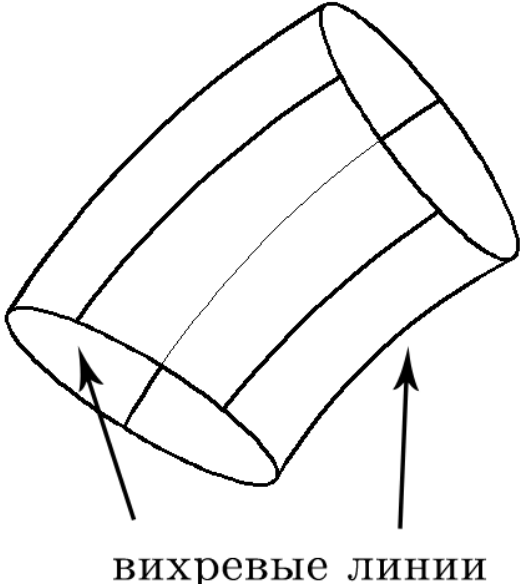
\includegraphics[width=\linewidth]{13/vihre_trubka.png}
        \captionof{figure}{Вихревая трубка}
    \end{minipage}\hfill
    \begin{minipage}{0.66\linewidth}
        \centering
        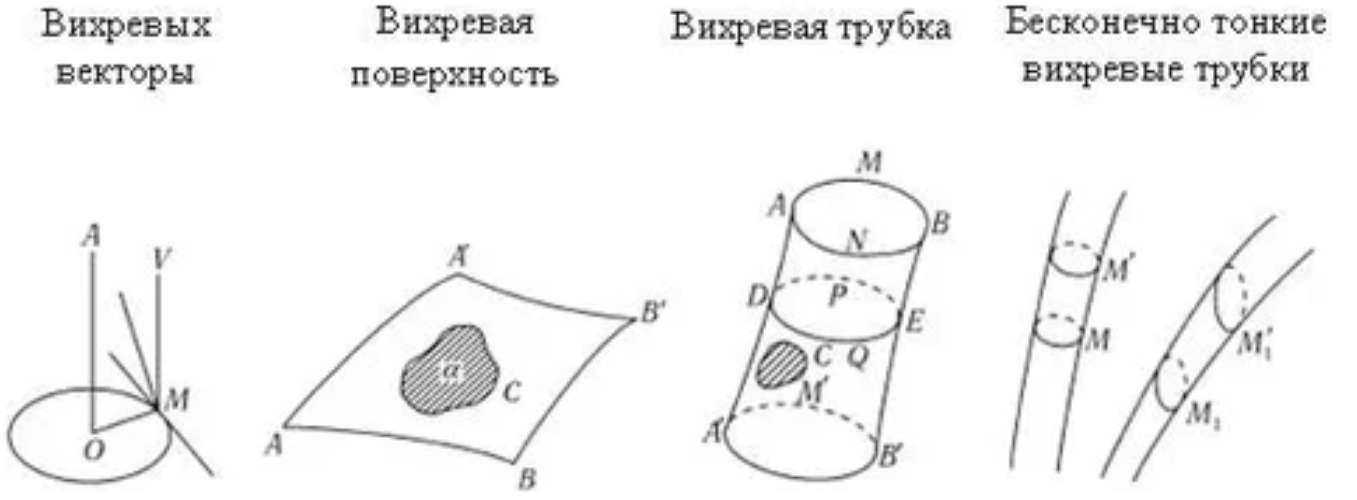
\includegraphics[width=\linewidth]{13/vihre_all.png}
        \captionof{figure}{}
    \end{minipage}
\end{figure}
\item \textbf{Интенсивность вихревой трубки} — поток ротора скорости внутри трубки через поперечное сечение $S$.
$$
\Gamma = \iint\limits_{S}\vec{\omega}d\vec{s}  =\iint\limits_{S}\vec{\omega}_nds =\text{(по теореме Стокса)} = \frac{1}{2}  \oint  \limits_{\partial S}\vec{v}d\vec{l}$$
\end{enumerate}
\begin{center}
	\textit{\underline{Уравнение эволюции завихрённости}}
\end{center}
$\vec{\omega} = \frac{1}{2}rot\vec{v} \Rightarrow div \vec{\omega}= 0$.\\
Возьмём $rot$ от уравнения движения в форме Громека-Лэмба и получим:
\begin{equation}
\label{vihre_eq_evol}
\frac{\partial \vec{\omega}}{\partial t} = rot(\vec{v}\times \vec{\omega})
\end{equation}
\begin{center}
	\textit{\underline{Первая кинематическая теорема Гельмгольца}}
\end{center}
\begin{theorem}
Интенсивность вихревой трубки одинакова по любому контуру, опоясывающему вихревую трубку.
\end{theorem}
\begin{proof}
\begin{minipage}{0.25\linewidth}
    \centering
    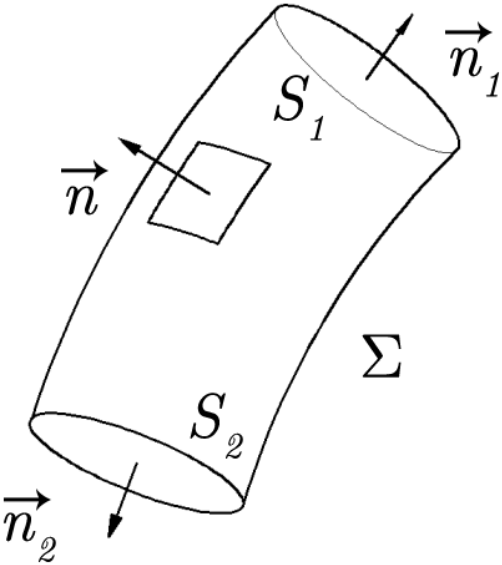
\includegraphics[width=\linewidth]{13/vihre_sech.png}
    \captionof{figure}{}
\end{minipage}
$0 = \int\limits_Vdiv \vec{\omega}dV = \int\limits_{S_1+S_2+\Sigma} \omega_ndS =\\ \text{(нормали противонаправлены и проекция\ }\omega_n \text{ на боковой поверхности, где вихревые линии, равна 0)} \\= -\int\limits_{S_1} \omega_ndS + \int\limits_{S_2} \omega_ndS + 0 = \Gamma_2 - \Gamma_1$.\\
\end{proof}
\begin{addition}
Вихревая линия получается из вихревой трубки с помощью предельного перехода при $S\xrightarrow[]{}0$.
\end{addition}
\begin{center}
	\textit{\underline{Вторая кинематическая теорема Гельмгольца}}
\end{center}
\begin{theorem}
Пусть задана вихревая трубка (или в частном случае вихревая линия). Тогда она либо замкнута, либо начинается и заканчивается на бесконечности.
\end{theorem}
\begin{proof}
(От противного) Пусть у неё есть начало, тогда в начале интенсивность нулевая. Однако из первой кинематической теоремы Гельмгольца следует, что интенсивность всюду должна быть нулевая. Противоречие.
\end{proof}
\begin{center}
	\textit{\underline{Теорема Томпсона}}
\end{center}
\begin{theorem}
В предположениях баротропности и потенциальности внешних сил выполнено соотношение \ref{vihre_eq_evol}.
Пусть линия $L$ является Лагранжевым контуром (т.е. вморожена в среду и двигается с её скоростью).
Тогда интенсивность жидкого контура остаётся постоянной.
\end{theorem}
\begin{proof}
\begin{minipage}{0.35\linewidth}
    \centering
    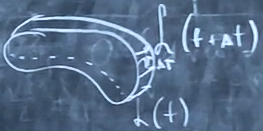
\includegraphics[width=\linewidth]{13/Tompson.png}
    \captionof{figure}{}
\end{minipage}
$\Gamma = \frac{1}{2}  \oint  \limits_{L}\vec{v}d\vec{l} = \iint\limits_{S}\vec{\omega}d\vec{s}$.\\
$$\frac{d\Gamma}{dt} =
\lim\limits_{\Delta t \xrightarrow[]{} 0} \frac{
\oint  \limits_{L(t + \Delta t)}\vec{v}(\vec{r}, t + \Delta t)d\vec{l}
-
\oint  \limits_{L(t)}\vec{v}(\vec{r}, t)d\vec{l}
}{\Delta t}
=
\lim\limits_{\Delta t \xrightarrow[]{} 0} \frac{\Gamma(t+\Delta t) - \Gamma(t)}{\Delta t}.
$$

$$0 = \int\limits_Vdiv \vec{\omega}dV = -\int\limits_{S(t)} \vec{\omega}(\vec{r}, t) d\vec{S} + \int\limits_{S(t+\Delta t)} \vec{\omega}(\vec{r}, t) d\vec{S} + \int\limits_{S_{\text{бок}}} \vec{\omega}(\vec{r}, t) d\vec{S} \Rightarrow [d\vec{S} = d\vec{l}\times \vec{v}\Delta t] \Rightarrow$$
$$\Rightarrow 
\Gamma(t) = \int\limits_{S(t+\Delta t)} \vec{\omega}(\vec{r}, t) d\vec{S} + \oint\limits_{L} \vec{\omega}(\vec{r}, t)[d\vec{l}\times \vec{v}]\Delta t \Rightarrow \\$$
$$\Rightarrow  
\frac{d\Gamma}{dt} =
\lim\limits_{\Delta t \xrightarrow[]{} 0} \frac{
\int  \limits_{S(t + \Delta t)}[\vec{\omega}(\vec{r}, t + \Delta t) - \vec{\omega}(\vec{r}, t)]dS
-
\oint\limits_{L} \vec{\omega}(\vec{r}, t)[d\vec{l}\times \vec{v}]\Delta t
}{\Delta t}
=$$
$$=
\int\limits_S \frac{\partial\vec{\omega}}{\partial t}dS - \oint\limits_{L} \vec{\omega}(\vec{r}, t)[d\vec{l}\times \vec{v}] =$$
$$=
\int\limits_S \frac{\partial\vec{\omega}}{\partial t}dS - \oint\limits_{L} d\vec{l}[\vec{v}\times \vec{\omega}] = \text{(т. Стокса)} = \int\limits_S (\frac{\partial\vec{\omega}}{\partial t} - rot[\vec{v}\times\vec{\omega}])dS = 0,$$
$\text{\ в силу уравнения \ref{vihre_eq_evol} и произвольности контура.}
$
\end{proof}
\begin{center}
	\textit{\underline{Следствия теоремы Томпсона. Динамическая теорема Гельмгольца.Теорема Лагранжа.}}
\end{center}
\begin{theorem}
В условиях предыдущей теоремы пусть задана вихревая поверхность. Тогда при движении вихревая поверхность переходит в вихревую поверхность.
\end{theorem}
\begin{proof}
Для любого жидкого контура на этой поверхности интенсивность равна нулю (т.к. $\omega_n = 0$).\\
При движении интенсивность отаётся нулём. Значит, переходим в вихревую поверхность.
\end{proof}
\begin{addition}
Аналогично для вихревой линии и вихревой трубки.
\end{addition}
\begin{theorem}
В условиях предыдущей теоремы. Если в начальный момент времени $t_0$ отсутствовали вихри (движение потенциально), то их не будет и для любого $t_0 + \Delta t$ (движение всё ещё потенциально).
\end{theorem}
\begin{proof}
$\Gamma = 0, t = t_0 \Rightarrow \Gamma = 0,\ \forall t.$
\end{proof}

\newpage
\section{Безвихревое движение идеальной жидкости в трехмерном и в двумерном случаях. Примеры потенциалов. Применение теории функции комплексного переменного для решения задач плоского движения идеальной несжимаемой жидкости. Формула Жуковского.}

\begin{center}
	\textit{\underline{Напоминание.}}
\end{center}

\text{Рассматриваем случай несжимаемой жидкости, то есть такой что, $\rho = const$}

\text{Вспомним формулу Коши-Гельмгольца. Рассмотрим точку $M$ с координатами $x^{i}$ и ее малую окрестность , точка $M'$ с к-ми $x^{i} + dx^{i}$ . По формуле Тейлора имеем}

$$
\overrightarrow{v}(M^{'}) = \overrightarrow{v}(x^{i}) + \frac{\partial \overrightarrow{v}}{\partial x^{i}} dx^{i} = \overrightarrow{v}(M) + \nabla_{i} v_{j}dx^{i} \overrightarrow{\text{э}}^{j} = \overrightarrow{v}(M) + \frac{1}{2} (\nabla_i v_j + \nabla_j v_i) dx^{i} \overrightarrow{\text{э}}^{j} + \frac{1}{2} (\nabla_i v_j - \nabla_j v_i) dx^{i} \overrightarrow{\text{э}}^{j}
$$

где $\frac{1}{2} (\nabla_i v_j + \nabla_j v_i) = e_{ij}$ - компоненты тензора скорости деформации. Введем 
$$
\frac{1}{2} (\nabla_i v_j - \nabla_j v_i) = w_{ij}
$$
где $w_{ij}$ компоненты тензора вихря 

Введем вектор $w$, вектор вихря :
$$
w^{k} = \frac{1}{\sqrt{g}}w_{ij}
$$
где (i,j,k) - круговая перестановка (1,2,3)

Таким образом, формула Коши-Гельмагольца, это : 

$$
\overrightarrow{v}(M^{'}) = \overrightarrow{v}(M) + e_{ij} dx^{i} \overrightarrow{\text{э}}^{j} + [\overrightarrow{w} \times d\overrightarrow{r}]
$$

Движение называется вихревым, если $\overrightarrow{w} \neq 0$. Движение называется безвихревым, если $\overrightarrow{w} = 0$

\begin{center}
	\textit{\underline{Потенциал скорости.}}
\end{center}

Потенциал скорости - такая функция $\varphi$ , что для вектора скорости $\overleftrightarrow{v}$ выполнено 
$$
\overrightarrow{v} = grad \varphi, \ v_i = \nabla_i \varphi = \frac{\partial \varphi}{\partial x^i}
$$
в декартовых к-тах
$$
v_x = \frac{\partial \varphi}{\partial x}, \ v_y = \frac{\partial \varphi}{\partial y}, \ v_z = \frac{\partial \varphi}{\partial z}
$$

\textbf{Утверждение.} $\overrightarrow{v} = grad \varphi \Leftrightarrow \overrightarrow{w} = 0$

\newpage
Уравнение неразрывности 
$$
\frac{\partial \rho}{\partial t} + div(\rho \overrightarrow{v}) = 0
$$
при $\rho = 1$  приобретает вид $div( \overrightarrow{v}) = 0 $ . Отсюда следует , что в несжимаемой жидкости потенциал скорости удовлетворяет уравнению Лапласа $\Delta \varphi = 0$

Граничные условия задаются разные , зачастую ставятся условия непротекания , то есть $v_n |_{\Sigma} = 0$. В свою очередь это соответствует системе 
$$
\Delta \varphi = 0
$$
$$
\frac{\partial \varphi}{\partial n} |_{\Sigma} = 0
$$

\begin{wrapfigure}{r}{0.2\textwidth}
	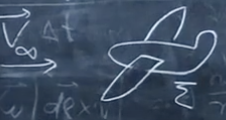
\includegraphics[width=0.2\textwidth]{14/pic_1.png}
	\caption{\label{ris:image14.1}}
\end{wrapfigure}

\begin{center}
	\textit{\underline{Примеры потенциалов.}}
\end{center}

Тут мы рассмотрим примеры различных функций $\varphi $. Рассматриваем задачу с набегающим с скоростью $\overrightarrow{v}_{\infty}$ однородным потоком на (как мы считаем покоящееся) тело.  Поверхность = $\Sigma$ и $\infty$  , т. о. $v_{\eta \leftarrow \infty} = v_\infty$ . Заметим, что задача линейная и потому складывая решения мы получим снова решение данной задачи.

1. Рассмотрим $\varphi_0 = \overrightarrow{v}_{\infty} x$, таким образом $grad \varphi = 0$ - все компоненты равны 0 . Это ситуация постоянного, однородного течения (течения на бесконечности). То , к чему стремится задача обтекания тела. Линии тока - прямые линии $z=y=const$

\begin{wrapfigure}{r}{0.2\textwidth}
	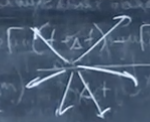
\includegraphics[width=0.2\textwidth]{14/pic_2.png}
	\caption{\label{ris:image14.2}}
\end{wrapfigure}

2. Рассмотрим $\varphi_1 = \frac{q}{r}, \ r = sqrt(x^2+y^2+z^2), \ q \ \text{это некоторая константа}$. Рассматриваем сферическую систему координат. Имеем в такой системе зависимость только от радиуса - имеем одну радиальную компоненту скорости $v_r = \frac {\partial \varphi_1 } {\partial r}= -\frac{\partial q}{\partial r^2}.$ Линии тока  на рисунке  2 - по напрвлению r $\theta = \varphi_1 = conts$. Если $q < 0$ это источник, если $q > 0$ это сток. $div \overrightarrow{v} = 0$, можем проинтегрировать по  сфере $Q = \int\limits_{S} \overrightarrow{v} d \overrightarrow{s} $ , получим $\varphi_1 =- \frac{Q}{4\Pi r}$

\begin{wrapfigure}{r}{0.2\textwidth}
	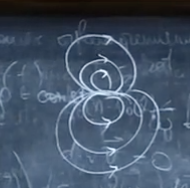
\includegraphics[width=0.2\textwidth]{14/pic_3.png}
	\caption{\label{ris:image14.3}}
\end{wrapfigure}

3. Можем рассмотреть $\varphi_2 = \frac{\partial \varphi_1} {\partial x}$.  Это диполь . Линии тока , получающиеся при данном потенциале, приведены на рисунке 3.


4. Можем сложить прошлые потенциалы и получить новый $\varphi_3 = \varphi_0 - \frac{\partial}{\partial x} \frac{Q}{4\Pi r}$. При некотором  $r$ данное выражение становится равно 0. Таким образом данный потенциал соответствует обтеканию шара

\newpage 

\begin{center}
	\textit{\underline{Примеры плоских течений. }}
	\\
	\textit{\underline{Применение теории функции комплексного
		 		переменного для решения задач плоского движения }}
	 \\
	 \textit{\underline{ идеальной несжимаемой жидкости. }}
\end{center}

Рассмотрим уравнение неразрывности в плоском случае 
$$
\frac{\partial u}{\partial x} + \frac{\partial v}{\partial y} = 0
$$
Уравнение отсутствия вихря 
$$
rot \overrightarrow{v} = 
\begin{vmatrix}
	\overrightarrow{e_x} & \overrightarrow{e_y}  & \overrightarrow{e_z} \\
	\frac{\partial }{\partial x} & \frac{\partial }{\partial y} & 0\\
	u & v & 0\
\end{vmatrix} = \overrightarrow{e_z} (\frac{\partial u}{\partial x} - \frac{\partial v}{\partial y} )
$$

\begin{wrapfigure}{r}{0.2\textwidth}
	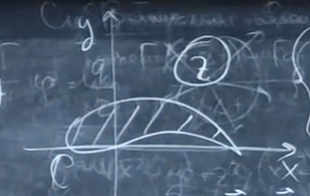
\includegraphics[width=0.2\textwidth]{14/pic_4.png}
	\caption{\label{ris:image14.4}}
\end{wrapfigure}

таким образом получаем условия Коши-Римана 
$$ \begin{cases}
\frac{\partial u}{\partial x} + \frac{\partial v}{\partial y} = 0  \ (\leftrightarrow \exists \psi)\\
\frac{\partial u}{\partial x} - \frac{\partial v}{\partial y}  = 0 \ (\leftrightarrow \exists \varphi)
\end{cases},$$

можем ввести комплескную переменную $x = x + i y$, т. о. $v = u + iv$, второе равенство из условий К-Р
$$ \begin{cases}
	\frac{\partial \varphi}{\partial x} = u  = \frac{\partial \psi}{\partial y}\\
	\frac{\partial \psi}{\partial y} = v = -\frac{\partial \varphi}{\partial x} 
\end{cases},$$
Таким образом получаем голоморфную функцию $w = \varphi + i \psi$. Если подставим в условие неразрывности , то получим $\Delta \varphi = 0$ , и при добавлении условия $\frac{\partial \varphi}{\partial n} |_C = 0 $ (условие непротекания), получим задачу Неймана. Здесь $C$ это просто контур.

В свою очередь если подставить $\psi $ в уравнение отсутствия вихря получим задачу Дирихле
$ \Delta \psi = 0 \quad \psi |_C = 0$



Рассмотрим дифференциал $d \psi$
$$
d \psi = \frac{\partial \psi}{\partial x}  dx +  \frac{\partial \psi}{\partial y}  dy = -vdx + udy
$$
\begin{wrapfigure}{r}{0.21\textwidth}
	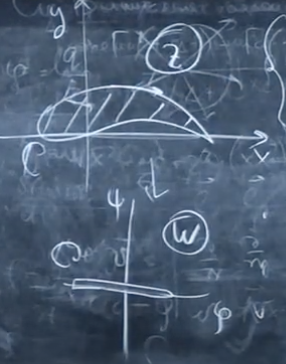
\includegraphics[width=0.21\textwidth]{14/pic_5.png}
	\caption{\label{ris:image14.5}}
\end{wrapfigure}
В свою очередь если $\psi = const $ (смысл линии - это линия тока), то $\frac{\partial x}{\partial u} = \frac{\partial y}{\partial v} $


Что такое \sout{бит}  функция w ? $w = \varphi x + i \psi$ - функция $z$, переводит конформно плоскость $z$ в плоскость $w$ , где $w=w(z)$ - комплексный потенциал течения

Во что перейдет контур $C$. По условию линия тока это константа. Пусть линия тока соответсвует $psi = q$, тогда контур в плоскости $w$ перейдет в отрезок (см. рисунок). То есть для решения задачи обтекания какого то плоского тела надо придумать функцию $w$, чтобы она сплющила тело до отрезка , лежащего на отрезке $\psi = 0$, на оси $\varphi$
$$$$
\newpage 

\begin{wrapfigure}{r}{0.15\textwidth}
	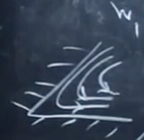
\includegraphics[width=0.15\textwidth]{14/pic_6.png}
	\caption{\label{ris:image14.6}}
\end{wrapfigure}



Рассмотрим каким течениям соответствуют какие  ситуации (потенциалы).

\begin{wrapfigure}{l}{0.15\textwidth}
	
\includegraphics[width=0.15\textwidth]{14/pic_7.png}
	\caption{\label{ris:image14.7}}
\end{wrapfigure}

1. Однородное течение, $w_0 = \overline{v}_{\infty} z$  , где $ \overline{v}_{\infty}  = const$ . Что такое $w'$ ? Это голоморфная функция , поэтому $w' = \frac{\partial \varphi}{\partial x} + i \frac{\partial \psi}{\partial x}  = u - iv = \overline{v}$


$w_0^{'} = \overline{v}_{\infty}$. В каждой точке скорость = const и равна $v_{\infty}$

2. $w_1 = z^n = r^n e^{i \theta n} = r^n(\cos(n \theta) + i \sin (n \theta) )$.  

Линии тока это $r^n \sin(n \theta) = const $ 

Рис 6 : $n > 1$ , течение в таком углу 

Рис 7: обтекание угла при $n < 1$ \\

В данном случае можем применить , например , инверсию . Можем наоборот , прямые линии (из плоскости w) перейти в течение (плоскость z)

$$ \begin{cases}
	w  = \frac{\partial u}{\partial z}\\
	z = -\frac{\partial u}{\partial w} 
\end{cases},$$

С помощью данного преобразования прямые линии на $w$ перейдут в окружности на $z$ . Причем окружности будут проходить через ноль. На самом деле получится диполь - см. рисунок 3.  

3. $z = e^{q w}, \ q \in \mathbb{R} , \quad w = \varphi + i \psi$. Таким образом $z = e^{q \varphi} e^{i q \psi}$, при этом $e^{i q \psi} = const$, радиус при этом пробегаем все диагонали $\varphi$

 Если $z$ чисто мнимое , то получаем течение - вихри. Соответствует рисунку 2.

\begin{center}
	\textit{\underline{Формула Жуковского.}}
\end{center}

\begin{wrapfigure}{r}{0.2\textwidth}
	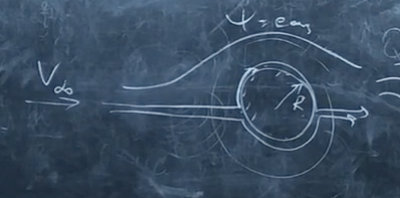
\includegraphics[width=0.2\textwidth]{14/pic_8.png}
	\caption{\label{ris:image14.8}}
\end{wrapfigure}

Рассмотрим $w=v_{\infty}(z + \frac{R^2}{z})$. Оно переводит окружность круга радиуса $R$ на некоторый отрезок . $w' = v_{\infty} ( 1 -  \frac{R^2}{z^2})$ , $w' \rightarrow v_{\infty} $ на бесконечности. Линии тока ведут себя как на рисунке 8. 

Также можем добавить к w функцию и рассмотреть следующий потенциал (круговые линии на рисунке 8 ) . Итого $w = v_{\infty}(z + \frac{R^2}{z}) + \frac{\Gamma}{2 \pi i} \ln z$. 

\begin{wrapfigure}{l}{0.15\textwidth}
	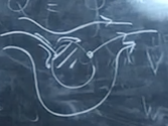
\includegraphics[width=0.15\textwidth]{14/pic_9.png}
	\caption{\label{ris:image14.9}}
\end{wrapfigure}
$$ $$

Вообще говоря $\Gamma$ произвольное, но надо выбрать единственное. По постулату Жуковского-Чаплыгина $\Gamma$ выбирается так чтобы в "острой", особенной точке скорость была равна нулю, то есть переходила в критическую точку. Таким образом можно выбрать единственное $\Gamma$. С гамма - циркуляцией получится картинка 9 с критической точкой (типа седло).

\newpage
\ \\

Рассмотрим произвольную функцию $w(z)$ и разложим в ряд Лорана $w' = ... + \frac{c_{-2}}{z^2} + \frac{c_{-1}}{z} + c_0 + c_1 z + c_2 z^2 + ... $. При устремлении z к бексонечности $w'$ должно получиться равным сопряженной скорости, таким образом $c_1 = c_2 = 0$, а $c_0 = \bar{v}_{\infty}$

Если взять циркуляцию от $w'$ , то получим $\Gamma = c_1 2 \pi i $ (по формуле) . $c_{-1} = \frac{\Gamma}{2 \pi i}$

\begin{wrapfigure}{r}{0.15\textwidth}
	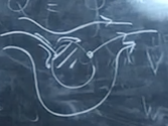
\includegraphics[width=0.15\textwidth]{14/pic_9.png}
	\caption{\label{ris:image14.10}}
\end{wrapfigure}
$$ $$

Чему равна сила , с действующая на данное тело ? 

Обозначим ее $R = X + i Y = - 	\oint \limits_{C} p \overrightarrow{n} d \overrightarrow{e} = - \oint \limits_{C} p e^(i\frac{pi}{2} + i\theta) d | \overrightarrow{e} |$ . Причем $p \in \mathbb{R}$

Что такое $dz$ ? $dz = e^{i \theta} d | \overrightarrow{e} |$, $w'$  в свою очередь, $w' = u -i \varv$ -  комплесносопряженная скорость 

Также вспомним интеграл Бернулли
$$ \begin{cases}
	p + p \frac{|v|^2}{2} = const \\
	v = u + i \varv
\end{cases},$$

Интеграл по кругу от константы по контуру равен нулю 

$- \oint \limits_{C} p e^(i\frac{pi}{2} + i\theta) d | \overrightarrow{e} | = -i \oint  \limits_{C} p dz = \frac{p i}{2} \oint  \limits_{C} |v|^2 dz =  \frac{p i}{2} \oint  \limits_{C} w' \bar{w}' d z$

Далее подробнее рассмотрим $w'$ , $\bar{w}' = v, \ \bar{d z} = e^{-i \theta} |d \overrightarrow{e} |$

$\bar{w}' \bar{dz} = |v| e^{i \theta} |d \overrightarrow{e} | e^{-i \theta} = w' dz$

$w' = ... + \frac{c_2}{z^2} + \frac{c_1}{z} + c_0 \ \rightarrow \ w'^2 = ... + \frac{2 c_1 c_0}{z} + ...$. Нас интересуют только вычеты , смотрим где $\frac{1}{z}$ 

В итоге получаем : 

$\bar{R} =  \frac{p}{2 i} \oint \limits_{C} \bar{w}'  w'  \bar{d z} =  \frac{p}{2 i} \oint \limits_{C} w'^2 dz =   \frac{p}{2 i} 2 c_{-1} c_0 2 \pi i = \rho c_{-1} c_0 2 \pi$

$ c_0 = \bar{v}_{\infty}$

$c_{-1} = \frac{\Gamma}{2 \pi i} $

Значит , $\bar{R} = - \rho \frac{\Gamma}{i} v_{\infty} $ (- на лекциях где-то потеряли, ну а я писал конспект по лекциям)

В итоге , Формула Жуковского 

$$
R = -i \rho v_{\infty} \Gamma
$$

Если скорость направлена в точности по оси x (то есть действительная часть равна 0) , то 

$X = 0$ - парадокс Даламбера , сила , действуюшая по направлению набегающей скорости равна нулю

$Y = -\rho v_{\infty} \Gamma $ - подъемная сила. Сила , напраленная перпендикулярно набегающей скорости , пропорциональна скорости и завихренности . Чем больше завихренности крыла, тем больше сила . 
\newpage
\section{Билет 15. Совершенный газ. Адиабатический процесс. Полная система уравнений, описывающая движение нетеплопроводного идеального газа. Скорость звука. Число Маха. Критерий сжимаемости в стационарном случае. Квазиодномерные стационарные течения. Сопло Лаваля}
	

\textbf{Совершенным газом} называется газ, для которого выполнено:

$1) p = \rho R T$ - уравнение Клапейрона

$2) u = c_v T + const, c_v = const$

Здесь $R = \dfrac{R_0}{\mu}$, $R_0$ - постоянная, одинаковая для всех газов.

$\mu$ - молекулярный вес газа

$c_v$ - удельная теплоемкость в процессах с постоянным объемом частиц.

Если воспользоваться уравнением неразрывности (1), уравнением движения (2) и вторым законом термодинамики (3), 
x   то мы получим замкнутую систему уравнений для определения неизвестных функций $\rho, v, s$:
$$\dfrac{d \rho}{d t} + \rho \,div\, v = 0 $$
  $$  \rho \dfrac{d v}{d t} = \rho F - grad p $$
   $$ T \dfrac{d s}{d t} = q^{e}$$

Процесс называется \textbf{Адиабатическим}, если нет притока тепла ни к одной частице, то есть $q^{e} = 0$.

В случае, если процесс адиабатаический, то тогда $\dfrac{d s}{d t} = 0$, где $s$ - энтропия. Мы считаем, что $s = s(p,\rho)$, тогда можно сказать, что $p = p (s, \rho)$. Тогда $d p = \left(\dfrac{d p}{d s}\right)d s + \left(\dfrac{d p}{d \rho}\right) d \rho$. Производную $\left(\dfrac{d p}{d \rho}\right)$ обозначают $a^2$. Используя условие $\dfrac{d s}{d t} = 0$ получим, что $\dfrac{d p}{d t} = a^2 \dfrac{d \rho}{d t}$.

Если задана внутренняя энергия $u = u (\rho, s)$, то $p = \rho^2 \dfrac{d u}{d \rho}$ и $T d s = d u$. Тогда получаем : $d u = \dfrac{p}{\rho^2}d \rho + T d s$ - тождество Гиббса.

Подставим условия совершенного газа $ p = \rho R T$ и $u = c_v T + const, c_v = const$ и получим следующее выражение:
$$T d s = c_v d T - \dfrac{R T}{\rho}d \rho$$
Используя обозначение $\dfrac{R}{c_v} = \gamma - 1$ можно записать выражение для плотности энтропии совершенного газа: 
$$s = c_vln\dfrac{T}{\rho^{\gamma-1}} + C_1 = c_v ln\dfrac{p}{\rho^\gamma} + C$$

Полная система уравнений, описывающая движение нетеплопроводного идеального газа:
$$\dfrac{d \rho}{d t} + \rho \,div\, v = 0 $$
  $$  \rho \dfrac{d v}{d t} = \rho F - grad \,p $$
  $$c_v T\, ln\dfrac{p}{\rho^\gamma} = 0$$
  $$1) p = \rho R T$$

В случае адиабатического процесса $s = const$. Тогда $\dfrac{p}{\rho^\gamma} = const $. Значит $a^2 = \gamma \dfrac{p}{\rho}$ - скорость звука.

Наши допущения: газ идеальный, течение адиабатическое, стационарное и одномерное (квазистационарное и одномерное теченение). Пусть $S$ - сечение.
$$div\, \rho v = 0$$
$$\rho v S = const$$
Прдифференцировав последнее равенство получим $\dfrac{d \rho}{\rho} + \dfrac{d v}{v} + \dfrac{d S}{S} = 0$.
Вспомним, что $dp = a^2 d\rho$.
Уравнение движения Эйлера запишется в виде:$$v\, dv = -a^2 \dfrac{d \rho}{\rho}$$
В итоге получаем $(v^2 - a^2)\dfrac{d v}{v} = a^2 \dfrac{dS}{S}$. Следовательно $(M^2 - 1)\dfrac{d v}{v = \dfrac{d S}{S}}$.
\textbf{Число Маха} $M$ - это отношение величины скорости потока к скорости звука в рассматриваемой точке. $M = \dfrac{v}{a}$

Из уравнения ясно видна роль числа М как критерия сжимаемости: чем меньше М, тем меньше влияние изменения скорости  на относительное изменение объема.

1) Если M < 1 , знак dv противоположен знаку dS , то есть, при дозвуковом движении газа, так же, как для несжимаемой жидкости, с возрастанием площади сечения трубы скорость движения уменьшается, а при уменьшении сечения скорость увеличивается.

Если M > 1 , знак dv совпадает со знаком dS , то есть, при сверхзвуковом движении газа в сужающейся трубе движение замедляется, а в расширяющейся ускоряется. Поэтому для получения сверхзвуковой струи надо использовать специальный насадок, имеющий сужающуюся и расширяющуюся части (сопло Лаваля)


\newpage
\section{Билет 16. Вязкая жидкость. Закон Навье-Стокса. Уравнения Навье-Стокса. Полная система уравнения, описывающая движение вязкой несжимаемой жидкости. Течение Пуазейля. Течение Куэтта. Закон Фурье. Полная система уравнений, описывающая движение вязкого теплопроводного совершенного газа.}

\begin{center}
	\textit{\underline{Вязкая жидкость}}
\end{center}

\begin{defn}
	Жидкость или газ называются \textbf{вязкими}, если в них при движении, возможно касательные напряжения. В таком случае компоненты тензора напряжений в вязкой жидкости представляются в виде: $$p^{ij}=-pg^{ij} + \tau^{ij},  \tau^{ij} = \tau^{ij}(e_{kl}, T) ,$$
	где $p$-давление, $e_kl$ - компоненты тензора скоростей деформаций, $T$-температура. 
\end{defn}

\begin{defn}
	\textbf{Компонентами тензора вязких напряжений} называются $\tau^{ij}$.
\end{defn}

Заметим, что если жидкость покоится, то $\tau^{ij} = 0$.

\begin{defn}
	Жидкость или газ называются \textbf{линейно-вязкими (или ньютоновскими)}, если $\tau^{ij}$ являются линейными функциями компонент тензора скоростей деформации ($e_{kl}$), т.е.: $$\tau^{ij} = A^{ijkl}e_{kl}, $$ где $A^{ijkl}$-коэффиценты вязкости.
\end{defn}


Ньютон в своем опыте с двумя пластинами выявил такую характеристику жидкости или газа, как вязкость.  Это свойство жидкости проявляется лишь при ее движении. Допустим, что некоторое количество жидкости заключено между двумя плоскими неограниченными параллельными пластинами; расстояние между ними – $d$; скорость движения верхней пластины относительно нижней – $v_0$.

Опыт показывает, что слой жидкости, непосредственно прилегающий к стенке, прилипает к ней. Отсюда следует, что скорость движения жидкости, прилегающей к нижней стенке, равна нулю, а к верхней – $v_0$. Промежуточные слои движутся со скоростью, постепенно возрастающей от $0$ до $v_0$.

Чтобы перемещать одну пластину относительно другой, необходимо приложить к движущейся пластине некоторую силу $F$, равную силе сопротивления жидкости в результате внутреннего трения. Ньютон установил, что эта сила пропорциональна скорости $v_0$, поверхности соприкосновения $S$ и обратно пропорциональна расстоянию между пластинами $d$ т.е.:
$$F = \mu\frac{S v_0}{d}$$

\begin{figure}[H]
	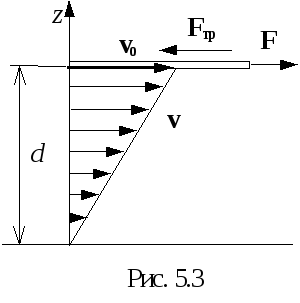
\includegraphics[width=0.4\textwidth]{16/newton_experiment.png}
\end{figure}


\begin{center}
	\textit{\underline{Закон Навье-Стокса}}
\end{center}


\begin{defn}
	\textbf{Изотропность} - совпадение свойства по всем направлениям. 
\end{defn}

\begin{theorem}[Э-132]Закон Навье-Стокса
	Для изотропных, линейно-вязких жидкостей верно следующее утверждение:
	$$\tau^{ij} = \lambda I_1(e)g^{ij}+2\mu e^{ij},$$ где $\lambda$, $\mu$ - коэффиценты вязкости, $I_1(e) = e_{ij}g^{ij}$ - первый инвариант тензора скоростей деформаций.
\end{theorem}


\begin{center}
	\textit{\underline{Уравнения Навье-Стокса}}
\end{center}

Уравнения движения линейно-вязких жикостей или газов называется уравнением Навье-Стокса. Они получаются из универсальных газовых уравнений: $$\rho\frac{dv^i}{dt} = \rho F^i + \nabla_{i}p^{ij}$$ подстановкой выражений для $p^{ij}$ и $\tau^{ij}$ и выведением уравнений покомпонентно.

Итоговое уравнение Навью-Стокса:

$$\frac{dv}{dt} = \hat{F} - \frac{1}{\rho}grad p + \frac{\lambda + \mu}{\rho}grad(div \hat{v}) + \frac{\mu}{\rho}\Delta \hat{v}$$


\begin{center}
	\textit{\underline{Полная система уравнения, описывающая движение вязкой несжимаемой жидкости}}
\end{center}


Полна система механических уравнений для несжимаемой линейно-вязкой жидкости с постоянными коэффицентами вязкости состоит из уравнения неразрывности, условия несжимаемости и уравнения Навье-Стокса:

\begin{equation} \label{eq:task}
	\begin{cases}
		\begin{array}{l}
			div \, \hat{v} = 0\\
			\frac{d\rho}{dt} = \frac{\partial \rho}{\partial t} + v^k\frac{\partial \rho}{\partial x^k} = 0\\
			\frac{dv}{dt} = \hat{F} - \frac{1}{\rho}grad\, p + \frac{\mu}{\rho}\Delta \hat{v}
		\end{array}
	\end{cases}
\end{equation}

\begin{center}
	\textit{\underline{Течение Пуазейля}}
\end{center}

\begin{defn}
	\textbf{Течение Пуазейля} - ламинарное течение жидкости через каналы в виде прямого кругового цилиндра или слоя между параллельными плоскостями. Течение Пуазёйля — одно из самых простых точных решений уравнений Навье — Стокса. Описывается законом Пуазёйля (также называемым законом Гагена — Пуазёйля или Хагена — Пуазёйля).
\end{defn}

\begin{figure}[H]
	\centering
	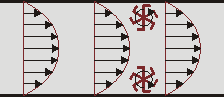
\includegraphics[width=0.4\textwidth]{16/poiseuille_profile.png}
\end{figure}

Течение Пуазёйля характеризуется параболическим распределением скорости по радиусу трубки. В каждом поперечном сечении трубки средняя скорость вдвое меньше максимальной скорости в этом сечении.


\begin{center}
	\textit{\underline{Течение Куэтта}}
\end{center}

\begin{defn}
	\textbf{Течение Куэтта} - ламинарное течение вязкой жидкости между двумя параллельными стенками (не обязательно прямолинейными), одна из которых двигается относительно другой. Течение происходит под действием сил вязкого трения, действующих на жидкость, и сдвигового напряжения параллельного стенкам.
\end{defn}



\newpage
\section{Билет 17. Безразмерные параметры, определяющие характер движения несжимаемой вязкой жидкости. Число Рейнольдса. Предельные случаи. Пограничный слой.}

Источник: \url{https://pstu.ru/files/2/file/kafedra/fpmm/of/Kolesnichenko_V.I._Vvedenie_v_mehaniku_nesjimaemoyi_jidkosti.pdf}

\subsection{Безразмерные параметры}
Будем рассматривать для примера двумерное (плоское) движение и теплоперенос вязкой несжимаемой жидкости. Оно характеризуется системой уравнений:
\begin{equation}
    \begin{cases}
        \frac{\partial v_x}{\partial t} + v_x\frac{\partial v_x}{\partial x} + v_y\frac{\partial v_x}{\partial y} = -\frac{1}{\rho} \frac{\partial p}{\partial x} + \nu (\frac{\partial^2 v_x}{\partial x^2} + \frac{\partial^2 v_x}{\partial y^2})\\

        \frac{\partial v_y}{\partial t} + v_x\frac{\partial v_y}{\partial x} + v_y\frac{\partial v_y}{\partial y} = -\frac{1}{\rho} \frac{\partial p}{\partial y} + \nu (\frac{\partial^2 v_y}{\partial x^2} + \frac{\partial^2 v_y}{\partial y^2})\\

        \frac{\partial v_x}{\partial x} + \frac{\partial v_y}{\partial y} = 0\\

        \frac{\partial T}{\partial t} + v_x\frac{\partial T}{\partial x} + v_y\frac{\partial T}{\partial y} = \alpha(\frac{\partial^2 v_x}{\partial x^2} + \frac{\partial^2 v_x}{\partial y^2})\\
    \end{cases}
\end{equation}

Здесь:
\begin{enumerate}
    \item[\textbullet] $v$ - скорость потока
    \item[\textbullet] $p$ - давление
    \item[\textbullet] $\nu$ - кинематическая вязкость 
    \item[\textbullet] $\alpha$ - коэффициент температуропроводности
    \item[\textbullet] $T$ - температура
\end{enumerate}

\bigskip
Введем следующие характерные величины:
\begin{enumerate}
    \item[\textbullet] $L$ - геометрический размер, например, диаметр цилиндрического канала
    \item[\textbullet] $v_0$ - скорость, например, скорость на оси канала или набегающего потока
    \item[\textbullet] $p_0$ - давление, например, на входе в канал
    \item[\textbullet] $t_0 = \frac{L}{v_0}$ - временной масштаб задачи
    \item[\textbullet] $T_h - T_c$ -  разность температур, например, горячей и холодной стенок полости
\end{enumerate}

С помощью введенных характерных величин определим безразмерные переменные (будем обозначать их буквами с верхним значком «тильда»), которые свяжем со старыми размерными переменными:

$$\Tilde{x} = \frac{x}{L},\; \Tilde{y} = \frac{y}{L},\; \Tilde{v_x} = \frac{v_x}{v_0},\; \Tilde{v_y} = \frac{v_y}{v_0},\; \Tilde{p} = \frac{p}{p_0},\; \Tilde{t} = t_0\frac{v_0}{L},\; \Tilde{\theta} = \frac{T - T_h}{T_h - T_c}$$

$$\frac{\partial}{\partial \Tilde{t}} = \frac{l}{v_0} \frac{\partial}{\partial t},\; \frac{\partial}{\partial \Tilde{x}} = l \frac{\partial}{\partial x},\; \frac{\partial^2}{\partial \Tilde{x}^2} = l^2 \frac{\partial}{\partial x^2}\;\; (and\; so\; on...)$$

Тогда обезразмеренное уравнение [1] нашей исходной системы переписывается в виде:

$$\frac{v_0L}{\nu} (\frac{\partial \Tilde{v_x}}{\partial \Tilde{t}} + \Tilde{v_x}\frac{\partial \Tilde{v_x}}{\partial \Tilde{x}} + \Tilde{v_y}\frac{\partial \Tilde{v_x}}{\partial \Tilde{y}}) = -\frac{p_0L}{\rho \nu v_0} \frac{\partial \Tilde{p}}{\partial \Tilde{x}} + (\frac{\partial^2 \Tilde{v_x}}{\partial \Tilde{x}^2} + \frac{\partial^2 \Tilde{v_x}}{\partial \Tilde{y}^2})$$

Коэффициент в левой части называется \textbf{числом Рейнольдса}:
$$Re = \frac{v_0L}{\nu}$$

Число Рейнольдса есть мера отношения сил инерции, действующих в потоке, к силам вязкости. При малых значениях $Re$ преобладают силы вязкости, при больших – силы инерции.

\bigskip
Преобразуем коэффициент в правой части:
$$\frac{p_0L}{\rho \nu v_0} = \frac{v_0L}{\nu} \cdot \frac{p_0}{\rho v_0^2} = Re \cdot Eu,$$
где коэффициент $$Eu = \frac{p_0}{\rho v_0^2}$$
называется \textbf{числом Эйлера}. Он описывает отношение между силами давления на единичный объём жидкости и инерционными силами.

\bigskip
Выразим $T = T_h + \theta (T_h - T_c)$ и обезразмерим уравнение [4] нашей исходной системы:

$$\frac{v_0L}{\alpha} (\frac{\partial \Tilde{\theta}}{\partial \Tilde{t}} + \Tilde{v_x}\frac{\partial \Tilde{\theta}}{\partial \Tilde{x}} + \Tilde{v_y}\frac{\partial \Tilde{\theta}}{\partial \Tilde{y}}) = (\frac{\partial^2 \Tilde{\theta}}{\partial \Tilde{x}^2} + \frac{\partial^2 \Tilde{\theta}}{\partial \Tilde{y}^2})$$

Коэффициент в левой части называется \textbf{числом Пекле}. Оно равно отношению конвективного теплопереноса к теплопроводному:
$$Re = \frac{v_0L}{\alpha}$$

Его также можно переписать в виде:
$$Re = \frac{v_0L}{\nu} \cdot \frac{\nu}{\alpha} = Re \cdot Pr,$$

где $Pr = \frac{\nu}{\alpha}$ называется \textbf{числом Прандтля}


\subsection{Пограничный слой}

Рассмотрим гидродинамические и тепловые процессы в пристенном слое жидкости. Скорость тончайшего слоя жидкости, непосредственно прилегающего к поверхности твердого тела, равна нулю, т.е. выполняется так называемое \textbf{условие прилипания}. 

Рассмотрим продольное обтекание плоской твердой поверхности тела безграничным потоком жидкости (см. рисунок). Пусть скорость набегающего потока постоянна и равна $v_0$ . Около пластины образуется слой заторможенной жидкости, в пределах которого скорость изменяется от нуля на поверхности до $v_0$ вдали от тела. Этот слой называется гидродинамическим \textbf{пограничным слоем}.

\begin{figure}[h]
    \centering
    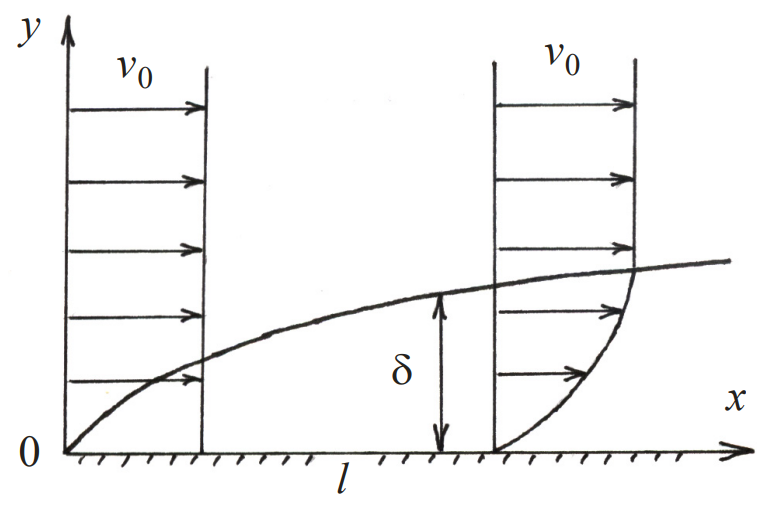
\includegraphics[scale=0.5]{17/fig_17_1.png}
    \caption{Пограничный слой}
\end{figure}

Толщина пограничного слоя $\delta$ – понятие довольно условное, так как резкого перехода от погранслоя к течению вне слоя
нет. Поэтому принимают под $\delta$ такое расстояние от стенки, при котором $v_x$ отличается от $v_0$ на заданную малую величину $\epsilon << 1$, например, $v_x = (1-\epsilon)v_0$ при $y=\delta$. Если $l$ – характерная длина пластины вдоль оси $OX$, то справедливо неравенство $\delta << l$.

\bigskip
При омывании пластины поток жидкости как бы разделяется на две части: пограничный слой, для которого справедливо условие
$$\frac{\partial v_x}{\partial y}\Big|_{y<\delta} \neq 0$$

и внешний поток, в котором $\frac{\partial v_x}{\partial y} = 0$; $v_x = v_0$ при $y \geq \delta$.

\bigskip
Во внешнем потоке, где число Рейнольдса $Re >> 1$, преобладают силы инерции, вязкостные силы здесь не проявляются, т.е. жидкость можно считать идеальной. Напротив, в пограничном слое силы вязкости и инерционные силы соизмеримы.

Явления, происходящие в пограничном слое, служат источником гидродинамического сопротивления при движении тел в жидкостях.

\bigskip
Распишем уравнения движения для двумерного стационарного потока жидкости:

\begin{equation}
    \begin{cases}
        v_x\frac{\partial v_x}{\partial x} + v_y\frac{\partial v_x}{\partial y} = -\frac{1}{\rho} \frac{\partial p}{\partial x} + \nu (\frac{\partial^2 v_x}{\partial x^2} + \frac{\partial^2 v_x}{\partial y^2})\\

        v_x\frac{\partial v_y}{\partial x} + v_y\frac{\partial v_y}{\partial y} = -\frac{1}{\rho} \frac{\partial p}{\partial y} + \nu (\frac{\partial^2 v_y}{\partial x^2} + \frac{\partial^2 v_y}{\partial y^2})\\

        \frac{\partial v_x}{\partial x} + \frac{\partial v_y}{\partial y} = 0\\
    \end{cases}
\end{equation}

Ввиду малости толщины пограничного слоя $\delta$ принимаем, что поперек него давление не изменяется ($\frac{\partial p}{\partial y} = 0$). Также будем рассматривать так называемое \textbf{безградиентное течение}, в котором в области пограничного слоя $\frac{\partial p}{\partial x} = 0$.

Проведём оценку порядков величин и слагаемых, входящих в рассматриваемую систему:
$$x = O(l),\; y = O(\delta),\; v_x = O(v_0)$$
$$\frac{\partial}{\partial x} = O(\frac{1}{l}),\; \frac{\partial^2}{\partial x^2} = O(\frac{1}{l^2}),\; \frac{\partial}{\partial y} = O(\frac{1}{\delta}),\; \frac{\partial^2}{\partial y^2} = O(\frac{1}{\delta^2})$$

Оценим величину $v_y$. Из уравнения неразрывности имеем $O(\frac{\partial v_x}{\partial x}) = O(\frac{\partial v_y}{\partial y})$ или $\frac{v_0}{l} = \frac{O(v_y)}{\delta}$, откуда получаем:
$$O(v_y) = v_0\frac{\delta}{l}$$

Оценим теперь порядки отдельных слагаемых первого уравнения системы:
$$v_x\frac{\partial v_x}{\partial x} = O(\frac{v_0^2}{l}),\; v_y\frac{\partial v_x}{\partial y} = O(v_0\frac{\delta}{l} \frac{v_0}{\delta}) = O(\frac{v_0^2}{l})$$
$$\nu \frac{\partial^2 v_x}{\partial x^2} = O(\nu \frac{v_0}{l^2}),\; \nu \frac{\partial^2 v_x}{\partial y^2} = O(\nu \frac{v_0}{\delta^2})$$

Видим, что отношение вязкостных членов равно $O(\nu \frac{v_0}{l^2}) : O(\nu \frac{v_0}{\delta^2}) = O(\frac{\delta^2}{l^2})$.

Поскольку для пограничного слоя $\delta << l$, то вязкостным членом можно пренебречь.

\bigskip
Оценим аналогично порядки отдельных слагаемых второго уравнения системы: 
$$v_x\frac{\partial v_y}{\partial x} = O(\frac{v_0^2}{l}\frac{\delta}{l}),\; v_y\frac{\partial v_y}{\partial y} = O(\frac{v_0^2}{l}\frac{\delta}{l})$$
$$\nu \frac{\partial^2 v_y}{\partial x^2} = O(\nu \frac{v_0}{l^2}\frac{\delta}{l}),\; \nu \frac{\partial^2 v_y}{\partial y^2} = O(\nu \frac{v_0}{\delta^2}\frac{\delta}{l})$$

Все члены уравнения в оценках порядков малости имеют сомножитель $\frac{\delta}{l} << 1$, следовательно, все эти члены малы по
сравнению с членами исходного уравнения. Вывод - в приближении погранслоя вторым уравнением системы полностью пренебрегают.

В итоге для плоского безградиентного стационарного течения вязкой жидкости в пограничном слое у плоской поверхности уравнения движения можно записать в следующем виде:

\begin{equation}
    \begin{cases}
        v_x\frac{\partial v_x}{\partial x} + v_y\frac{\partial v_x}{\partial y} = \nu \frac{\partial^2 v_x}{\partial y^2}\\

        \frac{\partial v_x}{\partial x} + \frac{\partial v_y}{\partial y} = 0\\
    \end{cases}
\end{equation}
\newpage
\section{Билет 18. Линейно упругое тело. Модуль Юнга, коэффициент Пуассона, коэффициненты Ламе. Связь этих коэффициентов между собой. Их физический смысл. Уравнения Ламе.}

\begin{center}
	\textit{\underline{Линейно упругое тело}}
\end{center}
\quad[Э-137]Среда называется \textbf{линейно-упругой}, или подчиняется закону Гука, если при постоянной температуре компоненты тензора напряжений являются линейными функциями компонент тензора деформации.

\quad Если в качестве начального (недеформированного) состояния выбрано состояние, в котором отсутствуют напряжения, т.е. $p^{ij}=0$ при $\epsilon_{ij}=0$, то эти линейные функции имеют вид: $$p^{ij}=A^{ijkl}\epsilon_{kl},$$
Коэффициенты $A^{ijkl}$ называются модулями упругости или упругими коэффициентами.

\begin{center}
	\textit{\underline{Закон Гука, модуль Юнга, коэф-ты Пуассона, Ламе, их связь}}
\end{center}


\quad Обобщённый закон Гука при произвольном деформировании при постоянной температуре для анизотропной среды: $$p^{ij}=A^{ijkl}\epsilon_{kl},$$
\quad Закон Гука для изотропной среды при изотермическом деформироваиии: $$p^{ij} = \lambda I_1(\epsilon)\delta^{ij}+2\mu \epsilon^{ij},$$
$I_1(\epsilon)$ - первый инвариант тензора деформаций, $\lambda, \mu$ - \textbf{коэффициенты Ламе}.

Из закона Гука имеем:
$$ \begin{cases}
p^{11} = \lambda I_1(\epsilon) + 2 \mu \epsilon_{11}\\
p^{22} = \lambda I_1(\epsilon) + 2 \mu \epsilon_{22}\\
p^{33} = \lambda I_1(\epsilon) + 2 \mu \epsilon_{33}
\end{cases},$$
Суммируем три вышенаписанных уравнения, получаем: $$I_1(p) = (3\lambda + 2\mu)I_1(\epsilon)  $$
Подставляем вместо $I_1(\epsilon)$, выражаем $\epsilon^{ij}$: $$\epsilon^{ij} = \frac{p^{ij}}{2\mu} - \frac{\lambda}{2\mu (3\lambda + 2\mu)}I_1(p)$$
Введём следующие обозначения: $$\frac{1}{2\mu} = \frac{1+\sigma}{E}, \qquad \frac{\lambda}{2\mu (3\lambda + 2\mu)}=\frac{\sigma}{E}$$
Выразим их через кожффициенты Ламэ (\textbf{связь коэффициентов}): $$E = \frac{\mu(3\lambda + 2\mu)}{\lambda + \mu}, \qquad \sigma = \frac{\lambda}{2(\lambda + \mu)}$$
E называется \textbf{модулем Юнга}, $\sigma$ - \textbf{коэффициентом Пуассона}.


\begin{center}
	\textit{\underline{Физический смысл коэффициентов}}
\end{center}
\begin{wrapfigure}{L}{0.5\textwidth}
\includegraphics[width=0.5\textwidth]{18/pic1.JPG}
\caption{1}
\label{ris:image1}
\end{wrapfigure}
\quad Рассмотрим простое растяжение стержня вдоль оси $x^1$ (-> \ref{ris:image1} <-), т.е. состояние, в котором $p^{11}\neq0$, а все остальные $p^{ij}=0$. Закон Гука для простого растяжения стержня имеет вид: $$\frac{F}{S} \sim \frac{\triangle l}{l_0} ,$$
F - растягивающая сила, S - площадь поперечного сечения стержня, $\triangle l$ - удлинение стержня, $l_0$ - начальная длина стержня. $\frac{F}{S} = p_{xx}$ (если ось х направлена по силе), а $\frac{\triangle l}{l_0} = \epsilon_{xx}$ при малых деформациях. Из формул выше получаем: $$\epsilon^{11} = \frac{1}{E}p^{11}$$

Таким образом, \textbf{модуль Юнга} E - коэффициент пропорциональности между напряжением $p^{11}=\frac{F}{S}$ и относительным удлинением $\epsilon^{11}=\frac{\triangle l}{l}$ при простом растяжении стержня.
\begin{wrapfigure}{R}{0.3\textwidth}
\includegraphics[width=0.3\textwidth]{18/pic2.JPG}
\caption{\label{ris:image2}2}
\end{wrapfigure}
Далее, из тех же формул, получаем, что при простом растяжении вдоль оси $x^1$ $$\epsilon^{22} = -\frac{\sigma}{E}p^{11}=-\sigma \epsilon^{11}$$
Обычно при растяжении стержень становится тоньше, т.е. $\epsilon^{22} < 0$ при $\epsilon^{11} > 0$. Таким образом, \textbf{коэффициент Пуассона} $\sigma$ - коэффициент пропорциональности между относительным сжатием в поперечном направлении и относительным удлинением в продольном направлении при простом растяжении стержня.

\quad Рассмотрим простой сдвиг (-> \ref{ris:image2} <-), т.е. состояние, в котором в декартовой системе координат $p^{12}\neq 0, \quad p^{21}=p^{12}$, а остальные компоненты $p^{ij}=0$. Тогда из закона Гука получаем: $$\epsilon^{12} = \frac{1+\sigma}{E}p^{12} = \frac{p^{12}}{2\mu}, \quad p^{12} = 2\mu \epsilon^{12}$$
В случае малых деформаций $$\epsilon^{12} = \frac{1}{2}\chi^{12},$$
где $\chi^{12}$ - изменение угла между волокнами, лежавшими до деформации вдоль осей $x^1$, $x^2$. Следовательно, коэффициент $\mu$ - это коэффициент пропорциональности между сдвигающими напряжением и изменением угла между соответствующими волокнами при простом сдвиге. Поэтому $\mu$ называют \textbf{модулем сдвига}. 

\begin{center}
	\textit{\underline{Уравнения Ламе}}
\end{center}
\quad Схема получения уравнений Ламе (Навье-Ламе) такова:
\begin{itemize}
\item В уравнениях движения выражаем $p^{ik}$ с помощью закона Гука через $\epsilon^{ik}$;

Уравнение движения в общем виде: $$\rho\frac{d\vec{v}}{dt} = \rho \vec{F} + \frac{\partial (p^{ij}\vec{e}_i)}{\partial x_j}$$
В случае, когда перемещения тела малы, выражение для левой части можно упростить: $$\vec{v} = \frac{d \vec{w}}{dt}, v^i = \frac{d w^i}{dt} = \frac{\partial w^i}{\partial t} + v^k \triangledown w^i \approx \frac{\partial w^i}{\partial t},$$
где $w^i$ - компоненты вектора перемещения. Т.е. с точностью до малых высшего порядка: $$\frac{d v^i}{dt} = \frac{\partial^2 w^i}{dt^2}$$
Уравнение движения в линейной теории упругости: $$\rho_0\frac{\partial^2 w^i}{\partial t^2} = \rho_0 F^i + \triangledown_k p^{ik}$$
\item Подставляем $\epsilon^{ik}$ через $\triangledown^i v^k$ ($\epsilon^{ik} = \frac{1}{2}(\triangledown^i w^k + \triangledown^k w^i)$).
\end{itemize}

\textbf{Уравнения Ламе в векторной форме:} $$\rho_0\frac{\partial^2 \vec{w}}{\partial t^2} = \rho_0\vec{F} + (\lambda + \mu)grad(div\vec{w}) + \mu \triangle \vec{w}$$


\newpage
\section{Билет 19. Постановка задач теории упругости в перемещениях и напряжениях. Граничные условия. Принцип Сен-Венана.}

\subsection{В перемещениях}
Если на границе тела заданы перемещения, удобно в качестве основных уравнений брать уравнения теории упругости в перемещениях, которые называются уравнениями Навье-Ламе. Они получаются из общих уравнений количества движения с использованием закона Гука и формул, выражающих компоненты тензора деформации через перемещения. Уравнения Навье-Ламе выглядят следующим образом:
$$
\rho_0\frac{\partial^2 w^i}{\partial t^2} = \rho_0 F^i + (\lambda + \mu)g^{ij}\nabla_j \mathrm{div} \vec{w} + \mu \Delta w^i
$$

Если на поверхности тела заданы перемещения, то из уравнений Навье-Ламе определяется вектор $w$ и этим решается задача о равновесии упругого тела в перемещениях. Напряжения при этом могут быть найдены согласно закону Гука. 

\subsection{В напряжениях}

При решении задачи в напряжениях, используются уравнения равновесия в напряжениях  $$\rho_0 F^i + \nabla_j p^{ij} = 0$$, эти три уравнения содержат шесть неизвестных компонент тензора напряжений и составляют незамкнутую систему. В некоторых случаях, например из симметрии задачи, можно заранее понять, что в эти уравнения входят только три неизвестные компоненты напряжений и если на границе известны $p_n$, то можно найти напряжения используя только эти три уравнения.

В общем случае, с помощью закона Гука из уравнений совместности деформаций можно получить дополнительные уравнения, которым должны удовлетворять компоненты тензора напряжений. Эти уравнения называются уравнениями Бельтрами-Мичелла, и выглядят следующим образом:
$$
\Delta p_{ij} + \frac{1}{1+\sigma} \frac{\partial^2 \wp}{\partial x^i \partial x^j}
$$
Причем в декартовых координатах $\wp = p_{11} + p_{22} + p_{33}$.

\newpage
\subsection{Граничные условия}

Граничные условия в задачах теории упругости бывают трёх оснонвх типов:
\begin{enumerate}
\item Граничные условия первого рода: задан вектор $\vec{w}$ на всей поверхности тела $\Sigma$
\begin{center}
$\vec{w}\mid_{\Sigma} = \vec{f}(x^i,t)$, где $\vec{f}$ - заданная функция
\end{center}

\item Граничные условия второго рода: на поверхности тела $\Sigma$ задан вектор напряжений $\vec{P_n}$ как функция времени и координат точек поверхности
\begin{center}
$\vec{P_n}\mid_{\Sigma} = \vec{\varphi}(x^i,t)$, где $\vec{\varphi}$ - заданная функция
\end{center}

\item Граничные условия третьего рода: на одной части поверхности тела  $\Sigma_w$ задан вектор $\vec{w}$, а на другой части  $\Sigma_p$ - $\vec{P_n}$
\begin{center}
$\vec{w}\mid_{\Sigma_w} = \vec{f}$ \ \ \ \ \  $\vec{P_n}\mid_{\Sigma_p} = \vec{\varphi}$
\end{center}
\end{enumerate}

\subsection{Принцип Сен-Венана}

\begin{wrapfigure}{R}{0.4\textwidth}
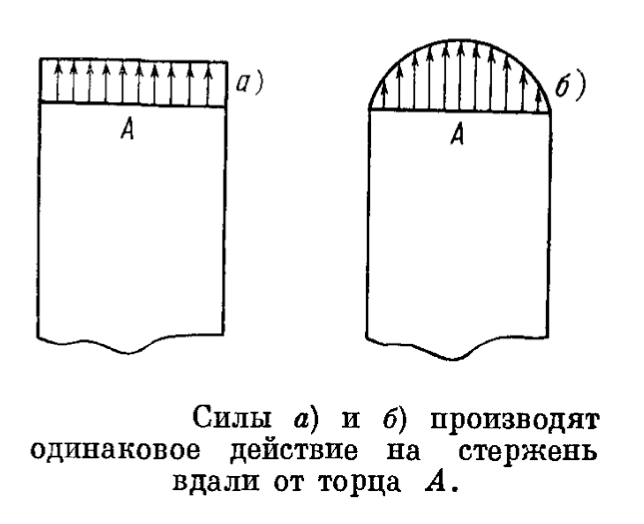
\includegraphics[width=0.4\textwidth]{19/sen_venan.png}
\end{wrapfigure}

Если в некоторой области внутри или на поверхности тела, малой по сравнению с основными размерами тела, на него действует система массовых или поверхностных сил и тело находится в равновесии, то в областях, удаленных от места приложения этих сил, деформированное и напряженное состояния определяются в основном только главным вектором и главным моментом этих сил и приближенно не зависят от детального характера распределения сил. Влияние деталей распределения сил практически сказывается только в непосредственной окрестности области их приложения.

\newpage
\section{Билет 20. Задача об изгибе балки.}

Рассмотрим упругую цилиндрическую балку произвольного поперечного сечения.

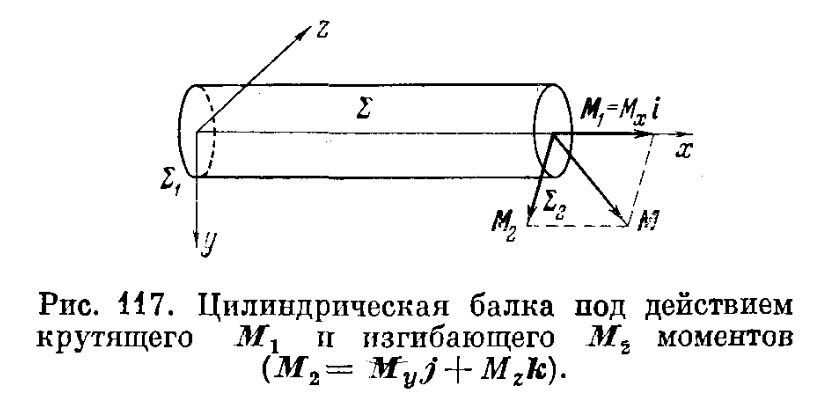
\includegraphics[scale=0.5]{20/t21_1.jpg}


\noindent Боковая поверхность балки $\Sigma$ не нагружена $\vec{p^n} = 0$.

\noindent На торце $\Sigma_2$ $\vec{p^n} \neq 0$, причем
$$\int_{\Sigma_2} {\vec{p^n} d{\sigma}} = 0,
\int_{\Sigma_2} (\vec{r} \times \vec{p^n}) d{\sigma} = \vec{M} \neq 0,$$

\noindent т.е. на торце $\Sigma_2$ балки действует пары сил с общим моментом $\vec{M}$. Балка по условию находиться в равновесии, поэтому на торце $\Sigma_1$

$$\int_{\Sigma_1} {\vec{p^n} d{\sigma}} = 0,
\int_{\Sigma_1} (\vec{r} \times \vec{p^n}) d{\sigma} = -\vec{M}$$

\noindent В общем случае момент $\vec{M}$ может иметь произвольное направление.

Выберем правую декартову систему координат $x$, $y$, $z$ так, чтобы ось $x$ была направлена по оси балки и проходила через центры тяжести поперечных сечений, а $y$, $z$ направлены по главным осям инерции поперечного сечения.

\noindent Тогда момент действующий на торце $\Sigma_2$ разложиться на три составляющие $\vec{M} = (M_x,M_y,M_z)$. Под действием $M_x$ балка будет закручиваться, а под действием моментов $M_y$, $M_z$ - изгибаться.

В силу линейности задачи общее решение получается как сумма решений трех задач: задачи о кручении под действием момента $M_x$ и двух задач об изгибе балки под действием моментов $M_y$ и $M_z$. Последние две задачи решаются аналогично.

Чистый изгиб балки $\vec{M} = (0,0,M_z)$


Распределение напряжений на торце $\Sigma_2$.
(Цитата лектора : "Угадываем решение") $\vec{p^n} = p_{11}\vec{e^1}$, $p_{11} = - \alpha y$. Проверим, что это решение на торцах удовлетворяет задаче.

Главный вектор: $ \int_{\Sigma_2} {\vec{p^n} d{\sigma}} = -\alpha \vec{e^1} \int_{\Sigma_2} {y d{\sigma}} = 0$, так как ось $x$ проходит через центр тяжести поперечного сечения.

$$ M_x = \int_{\Sigma_2} {(\vec{r} \times \vec{p^n})_x d{\sigma}} = 0,$$
\noindent так как $\vec{p^n}$ параллельно оси $x$,

$$ M_y = \int_{\Sigma_2} {(\vec{r} \times \vec{p^n})_y d{\sigma}} = \alpha \int_{\Sigma_2} {yz d{\sigma}} = 0,$$
\noindent так как оси $y$ и $z$ совпадают с главными осями инерции поперечного сечения,

$$ M = M_z = \int_{\Sigma_2} {(\vec{r} \times \vec{p^n})_z d{\sigma}} = \alpha \int_{\Sigma_2} {y^2 d{\sigma}} = \alpha J,$$
\noindent где J - момент инерции поперечного сечения относительно оси $z$. Решение удовлетворяет задаче, также найден коэффициент $\alpha$.

$$ \alpha = \frac{M}{J} $$

на другом торце аналогично, поверхностные силы распределены по закону $(\vec{p^n})_{\Sigma_1} = - (\vec{p^n})_{\Sigma_2}$

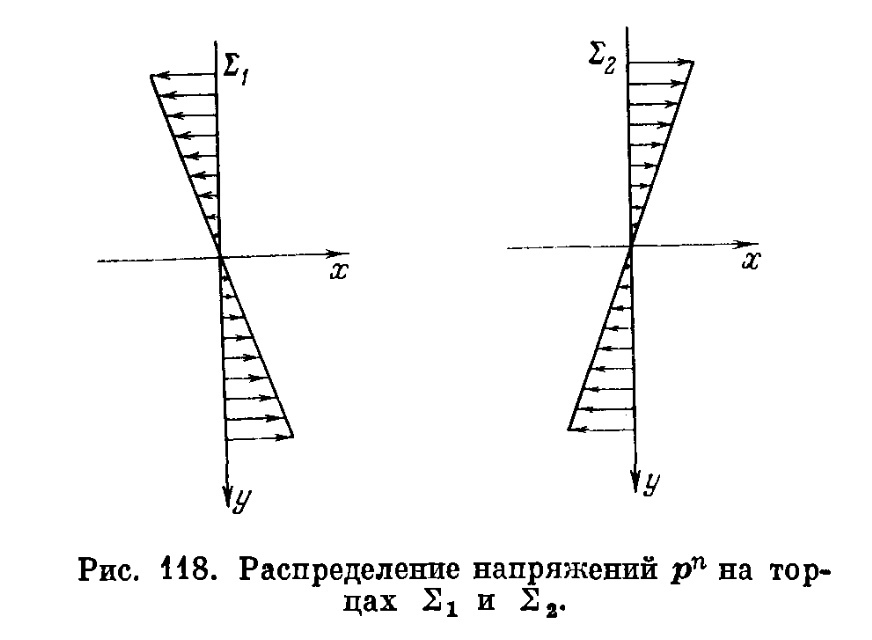
\includegraphics[scale=0.5]{20/t21_2.jpg}

Из принципа Сен-Венана следует, что полученное решение будет справедливо в части балки, достаточно удаленной от её торцов.

\noindent Тогда тензор напряжений во всех точках балки имеет вид:

\begin{equation*}
||p_{ij}|| = \left(
\begin{array}{ccc}
-\frac{M}{J}y & 0 & 0 \\
0 & 0 & 0 \\
0 & 0 & 0 \\
\end{array}
\right)
\end{equation*}

Закон Гука
$$ \varepsilon_{ij} = \frac{1}{E} \left[ (1+\sigma)p_{ij} - \sigma \mathfrak{P} g_{ij} \right] + \alpha (T-T_0)g_{ij} ,$$
где $\mathfrak{P}$ - первый инвариант тензора напряжений.

Примем, что температура во всех точках балки одинакова. Тогда по закону Гука можно вычислить компоненты тензора деформаций

\begin{equation}
\begin{array}{cc}
\varepsilon_{11} = -\frac{My}{EJ} = \frac{\partial w_1}{\partial x} & \varepsilon_{22} = \frac{\sigma My}{EJ} = \frac{\partial w_2}{\partial y} \\
\varepsilon_{33} = \frac{\sigma My}{EJ} = \frac{\partial w_3}{\partial z} & \varepsilon_{12} = \varepsilon_{23} = \varepsilon_{13} = 0
\end{array}
\end{equation}

Отсюда видно, что при чистом изгибе элементы балки, совпадающие с осью $x$, не испытывают удлинения, ни сжатия. Элементы, параллельные оси $x$, при $y>0$ сжимаются, а при $y<0$ растягиваются.

Из (1) можно найти вектор перемещения

\begin{equation}
\begin{array}{cc}
w_1 =& - \frac{Myx}{EJ} \\
w_2 =& \frac{M}{2EJ}[x^2 + \sigma (y^2 - z^2)] \\
w_3 =& \frac{\sigma Myz}{EJ}
\end{array}
\end{equation}


Любая точка балки $(x_0, y_0, z_0)$ переходит в точку с координатами $(x, y, z)$ по формулам

\begin{equation}
\begin{array}{cc}
x =& x_0 + w_1 = x_0 - \frac{My_0x_0}{EJ} \\
y =& y_0 + w_2 = y_0 + \frac{M}{2EJ}[x_0^2 + \sigma (y_0^2 - z_0^2)] \\
z =& z_0 + w_3 = z_0 + \frac{\sigma My_0z_0}{EJ}\\
\end{array}
\end{equation}

Тогда уравнение изогнутой оси балки $(y_0 = z_0 = 0)$ имеет вид
$$ y = \frac{M}{2EJ}x^2 $$

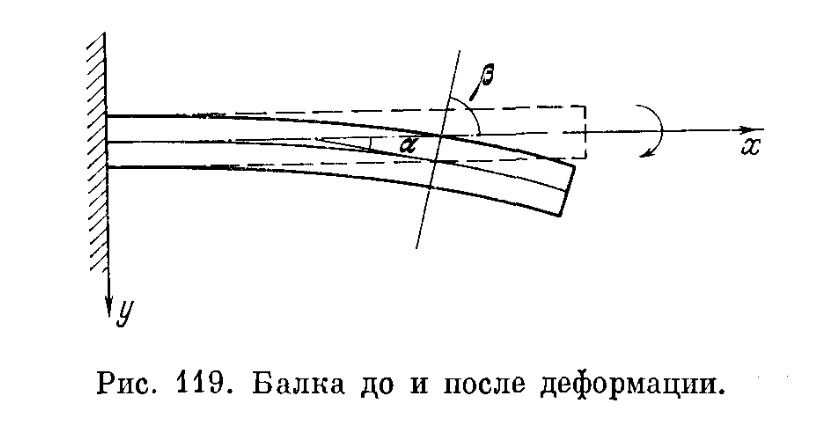
\includegraphics[scale=0.5]{20/t21_3.jpg}

\input {21/21_ticket.tex}

\newpage
\begin{thebibliography}{100}
	
\end{thebibliography}

\end{document}
